\chapter{iAPF Motion Planning}
\label{chap:iapf}

Chapter~\ref{chap:distance} closed with a continuous, sensor-free inter-arm distance signal
$D_{\text{inter}}$, and, as a first check that the signal was directly usable, integrated it with a
traditional artificial potential field controller under twist control
(Figure~\ref{fig:iapf_baselinetraj}). That controller was sufficient to demonstrate the distance
signal could drive a reactive collision-avoidance loop, but not to plan motion well: the traditional
two-force formulation's difficulties for asymmetric dual-arm coordination, workspace-sharing
deadlock and oscillation in cluttered scenes, were identified in Chapter~\ref{chap:lit_review} as
gap G4~\citep{surya2025iapf,sk2025competitive}.

\begin{figure}[htbp]
\centering
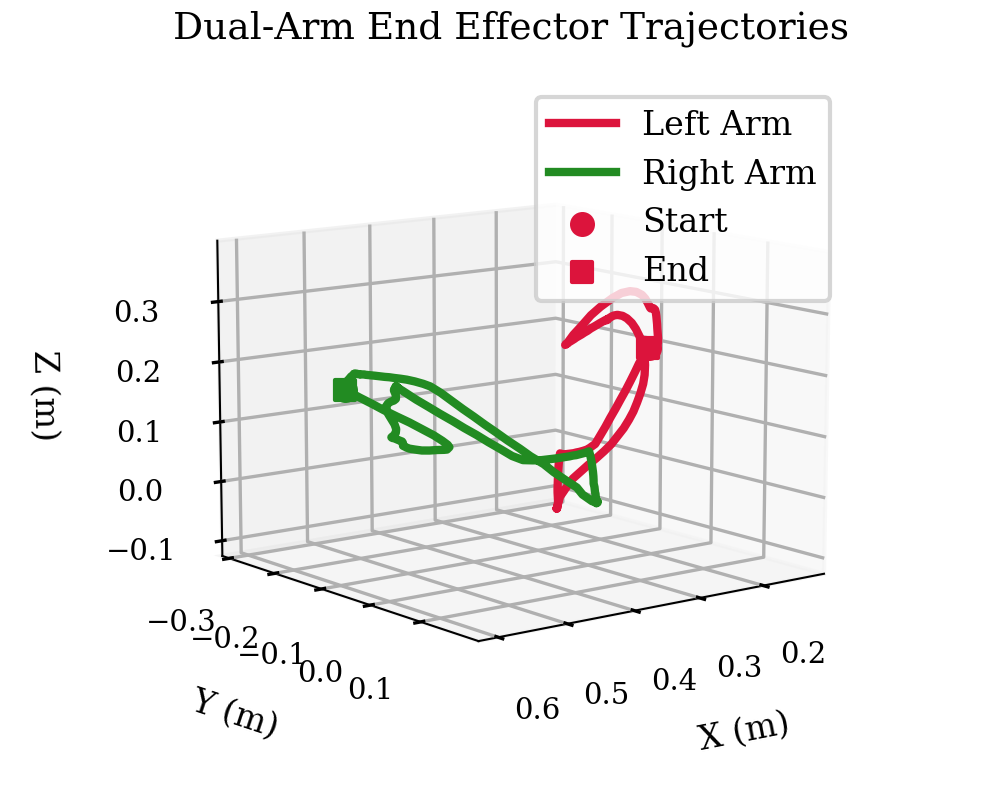
\includegraphics[width=0.85\linewidth]{Images/distanceMonitoring/trajectory_tracking.png}
\caption{Dual-arm end-effector trajectories through the home, pick, place, and return phases, under
the traditional artificial potential field controller used to validate that the inter-arm distance
signal of Chapter~\ref{chap:distance} is directly usable for reactive collision
avoidance~\citep{sk2025distance}.}
\label{fig:iapf_baselinetraj}
\end{figure}

This chapter presents the improved artificial potential field (iAPF) framework that closes gap G4: a
three-way equilibrium of goal attraction, inter-arm repulsion, and home-seeking forces, stabilized
by velocity-dependent damping, coupled to a PD-regulated angular velocity, with a priority-lock
coordination mechanism, validated experimentally across repeated dual-arm trials.
Sections~\ref{sec:iapf_architecture} through~\ref{sec:iapf_validation} present the framework as
originally introduced and published~\citep{surya2025iapf}, validated under a \emph{fixed}
object-to-arm assignment, nuts routed to the left arm and bolts to the right; that fixed assignment
is itself a separate limitation, gap G5, which Chapter~\ref{chap:task_allocation} takes up once the
motion-planning question this chapter answers is settled.

%% ============================================================
\section{System Architecture and Vision-Based Perception}\label{sec:iapf_architecture}
%% ============================================================

The iAPF framework was developed and validated on the same two-Kinova-Gen3-Lite cell used
throughout this thesis, augmented with a single globally mounted Intel RealSense D415 RGB-D camera.
Figure~\ref{fig:iapf_overall} summarizes the four components this chapter develops: inter-arm
distance calculation from forward kinematics, the three-way force equilibrium for collision
avoidance, vision-based pose estimation, and the resulting state-based asymmetric manipulation.

\begin{figure}[htbp]
\centering
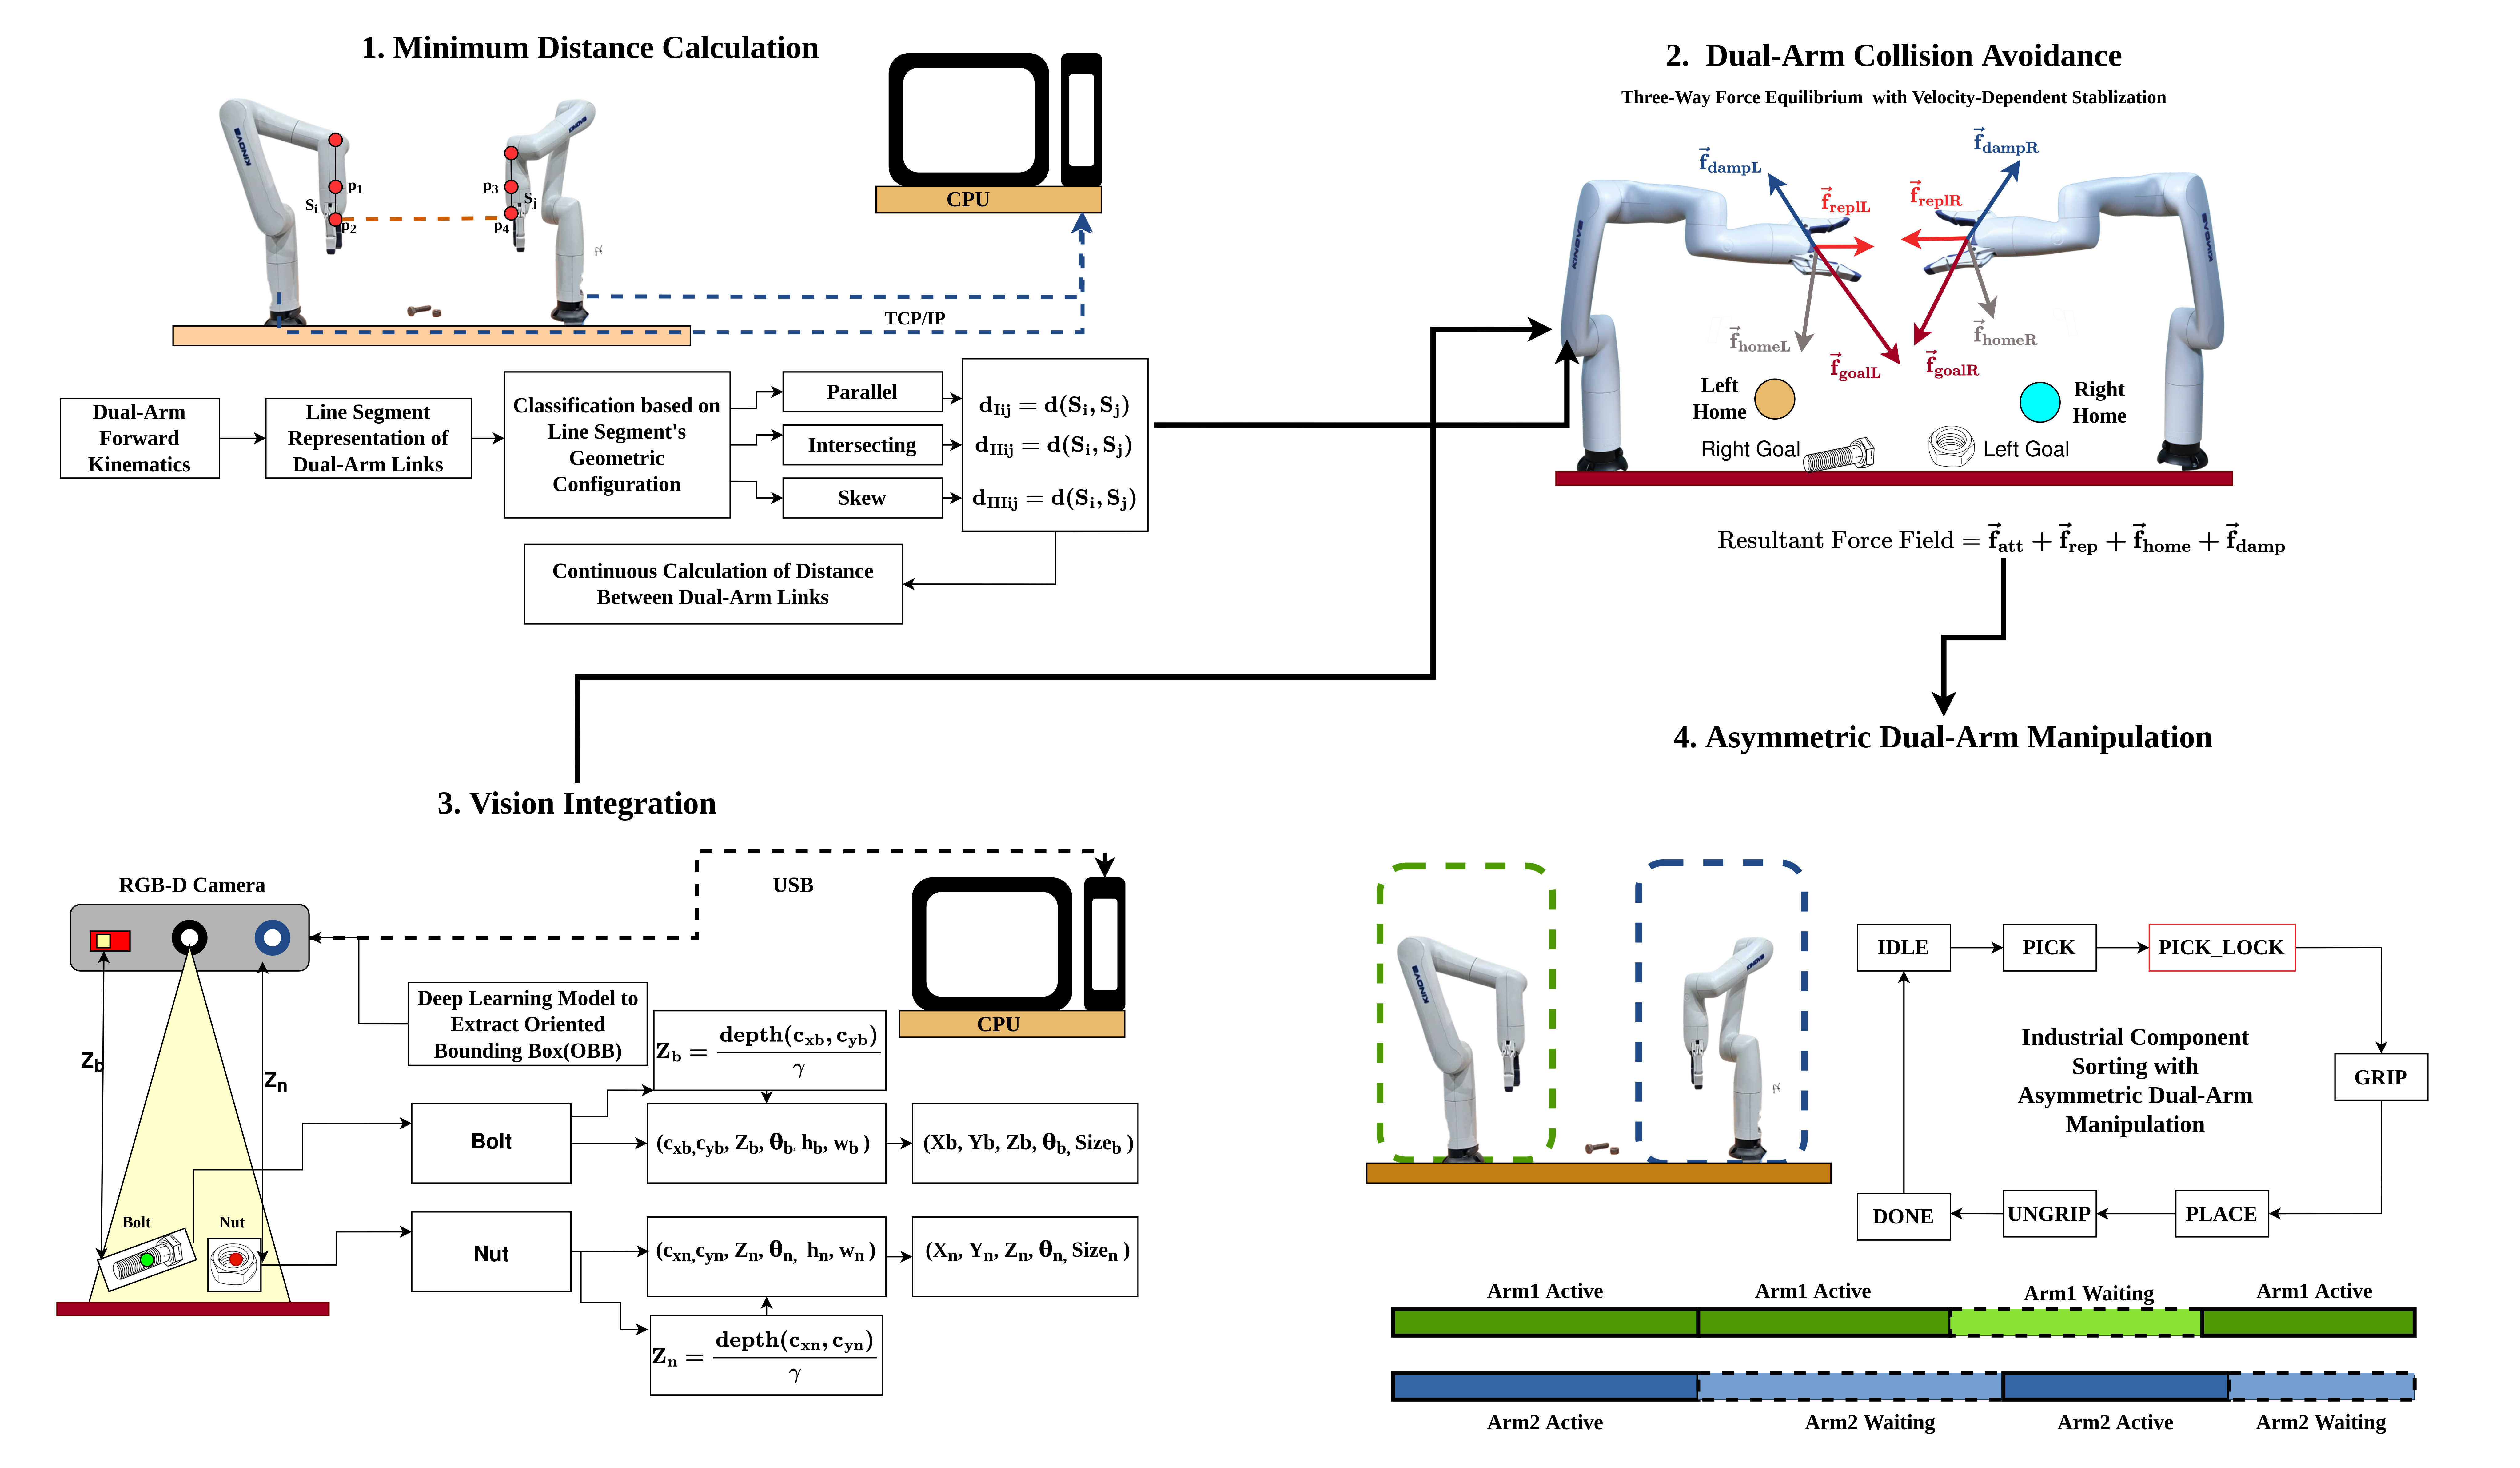
\includegraphics[width=\linewidth]{Images/iapf/overall_methodology.jpg}
\caption{Overall methodology for iAPF dual-arm motion planning: minimum distance calculation,
dual-arm collision avoidance via the three-way force equilibrium, vision integration, and the
resulting asymmetric dual-arm manipulation~\citep{surya2025iapf}.}
\label{fig:iapf_overall}
\end{figure}

Each arm's forward kinematics follows the D-H parameters already given in
Table~\ref{tab:dm_dh}, and each arm's link-to-link forward kinematics chain is exactly
Equation~\eqref{eq:sv_fwdkin}. As in Chapters~\ref{chap:shared_vision}
through~\ref{chap:iapf}, the left arm's base frame $B_L$ serves as the shared reference:
the camera is calibrated relative to the right arm's base, $T^{B_R}_{C}$, and the right arm's base is
related to the left by $T^{B_L}_{B_R}$, so that an object detected in the camera frame reaches the
shared reference frame by the same chained composition used throughout this thesis:
\begin{equation}
p^{B_L} = T^{B_L}_{B_R}\, T^{B_R}_{C}\, p^{C}.
\label{eq:iapf_objecttransform}
\end{equation}

Table~\ref{tab:iapf_comparison} summarizes how iAPF positions itself against the traditional and
enhanced APF variants reviewed in Chapter~\ref{chap:lit_review}: it is the only formulation among
these offering both empirically validated stability and real-time (10\,Hz) performance
simultaneously.

\begin{table}[htbp]
\centering
\caption{Comparison of iAPF against traditional and existing APF variants for industrial dual-arm
manipulation~\citep{surya2025iapf}.}
\label{tab:iapf_comparison}
\resizebox{\textwidth}{!}{%
\begin{tabular}{lllll}
\toprule
\textbf{Method} & \textbf{Force components} & \textbf{Stability guarantee} & \textbf{Real-time} & \textbf{Key limitation} \\
\midrule
Traditional APF~\citep{khatib1986real} & Attractive + repulsive & None & Moderate & Local minima in clutter \\
Enhanced APF (sampling-based) & Attractive + repulsive + sampling & Statistical ($95.2\%$) & Slow ($9.14$\,s) & High computational overhead \\
D-APF (UAV navigation) & Exponential + vertical priority & None & Moderate & Limited to UAV applications \\
Rotating APF & Attractive + rotating repulsive & Mathematical & Moderate & Single arm only, no coordination \\
\textbf{iAPF (proposed)} & Attractive + repulsive + home-seeking & \textbf{Empirically validated} & \textbf{Fast (10\,Hz)} & Dynamic obstacle adaptation \\
\bottomrule
\end{tabular}%
}
\end{table}

Object perception uses YOLOv8 with oriented bounding boxes (OBB)~\citep{yolov8}, selected over
instance-segmentation alternatives after a direct comparison on the same custom dataset,
Table~\ref{tab:iapf_modelcompare}: Detectron2 and the YOLO instance-segmentation variants all incur
either a substantially larger model or slower inference than the OBB detector, for a task, oriented
fastener localization, that does not require a per-pixel segmentation mask.

\begin{table}[htbp]
\centering
\caption{Model comparison for object detection on the custom nut/bolt dataset~\citep{surya2025iapf}.}
\label{tab:iapf_modelcompare}
\begin{tabular}{lcc}
\toprule
\textbf{Model} & \textbf{Model size (MB)} & \textbf{Inference (relative)} \\
\midrule
Detectron2 instance segmentation & 351.1 & 0.51 \\
YOLOv8 instance segmentation     & 20.0  & 15 \\
YOLOv11 instance segmentation    & 6.0   & 13 \\
\textbf{YOLOv8 OBB}              & \textbf{5.9} & \textbf{20} \\
\bottomrule
\end{tabular}
\end{table}

The custom dataset, 1230 images split 1120/80/30 into training, validation, and test sets and
ten-folded by augmentation, covers varying backgrounds, lighting, and both new and aged fasteners
(Figure~\ref{fig:iapf_datacollection}), reaching 20\,FPS inference at deployment. Following
detection, each object's OBB (Figure~\ref{fig:iapf_obb}) gives centroid $(c_u, c_v)$, orientation
$\theta$, and bounding-box width $h$ and
height $w$ in pixels. Position is recovered by the same pinhole back-projection as
Equation~\eqref{eq:vp_backproject}, and size by the same relation as
Equation~\eqref{eq:vp_pixel2metric}, both using the camera's principal point and focal lengths from
intrinsic calibration and the corrected depth $Z$. The resulting per-object feature is
$F_{\text{nut/bolt}} = [X, Y, Z, \theta, \text{size}]$. Since the gripper's own zero-orientation
does not coincide with the detected object frame, the desired gripper yaw is offset from the
detected angle,
\begin{equation}
\theta_{\text{gripper}} = 270^\circ - \theta,
\label{eq:iapf_gripperangle}
\end{equation}
ensuring the gripper approaches aligned with the fastener regardless of its detected orientation.

\begin{figure}[htbp]
\centering
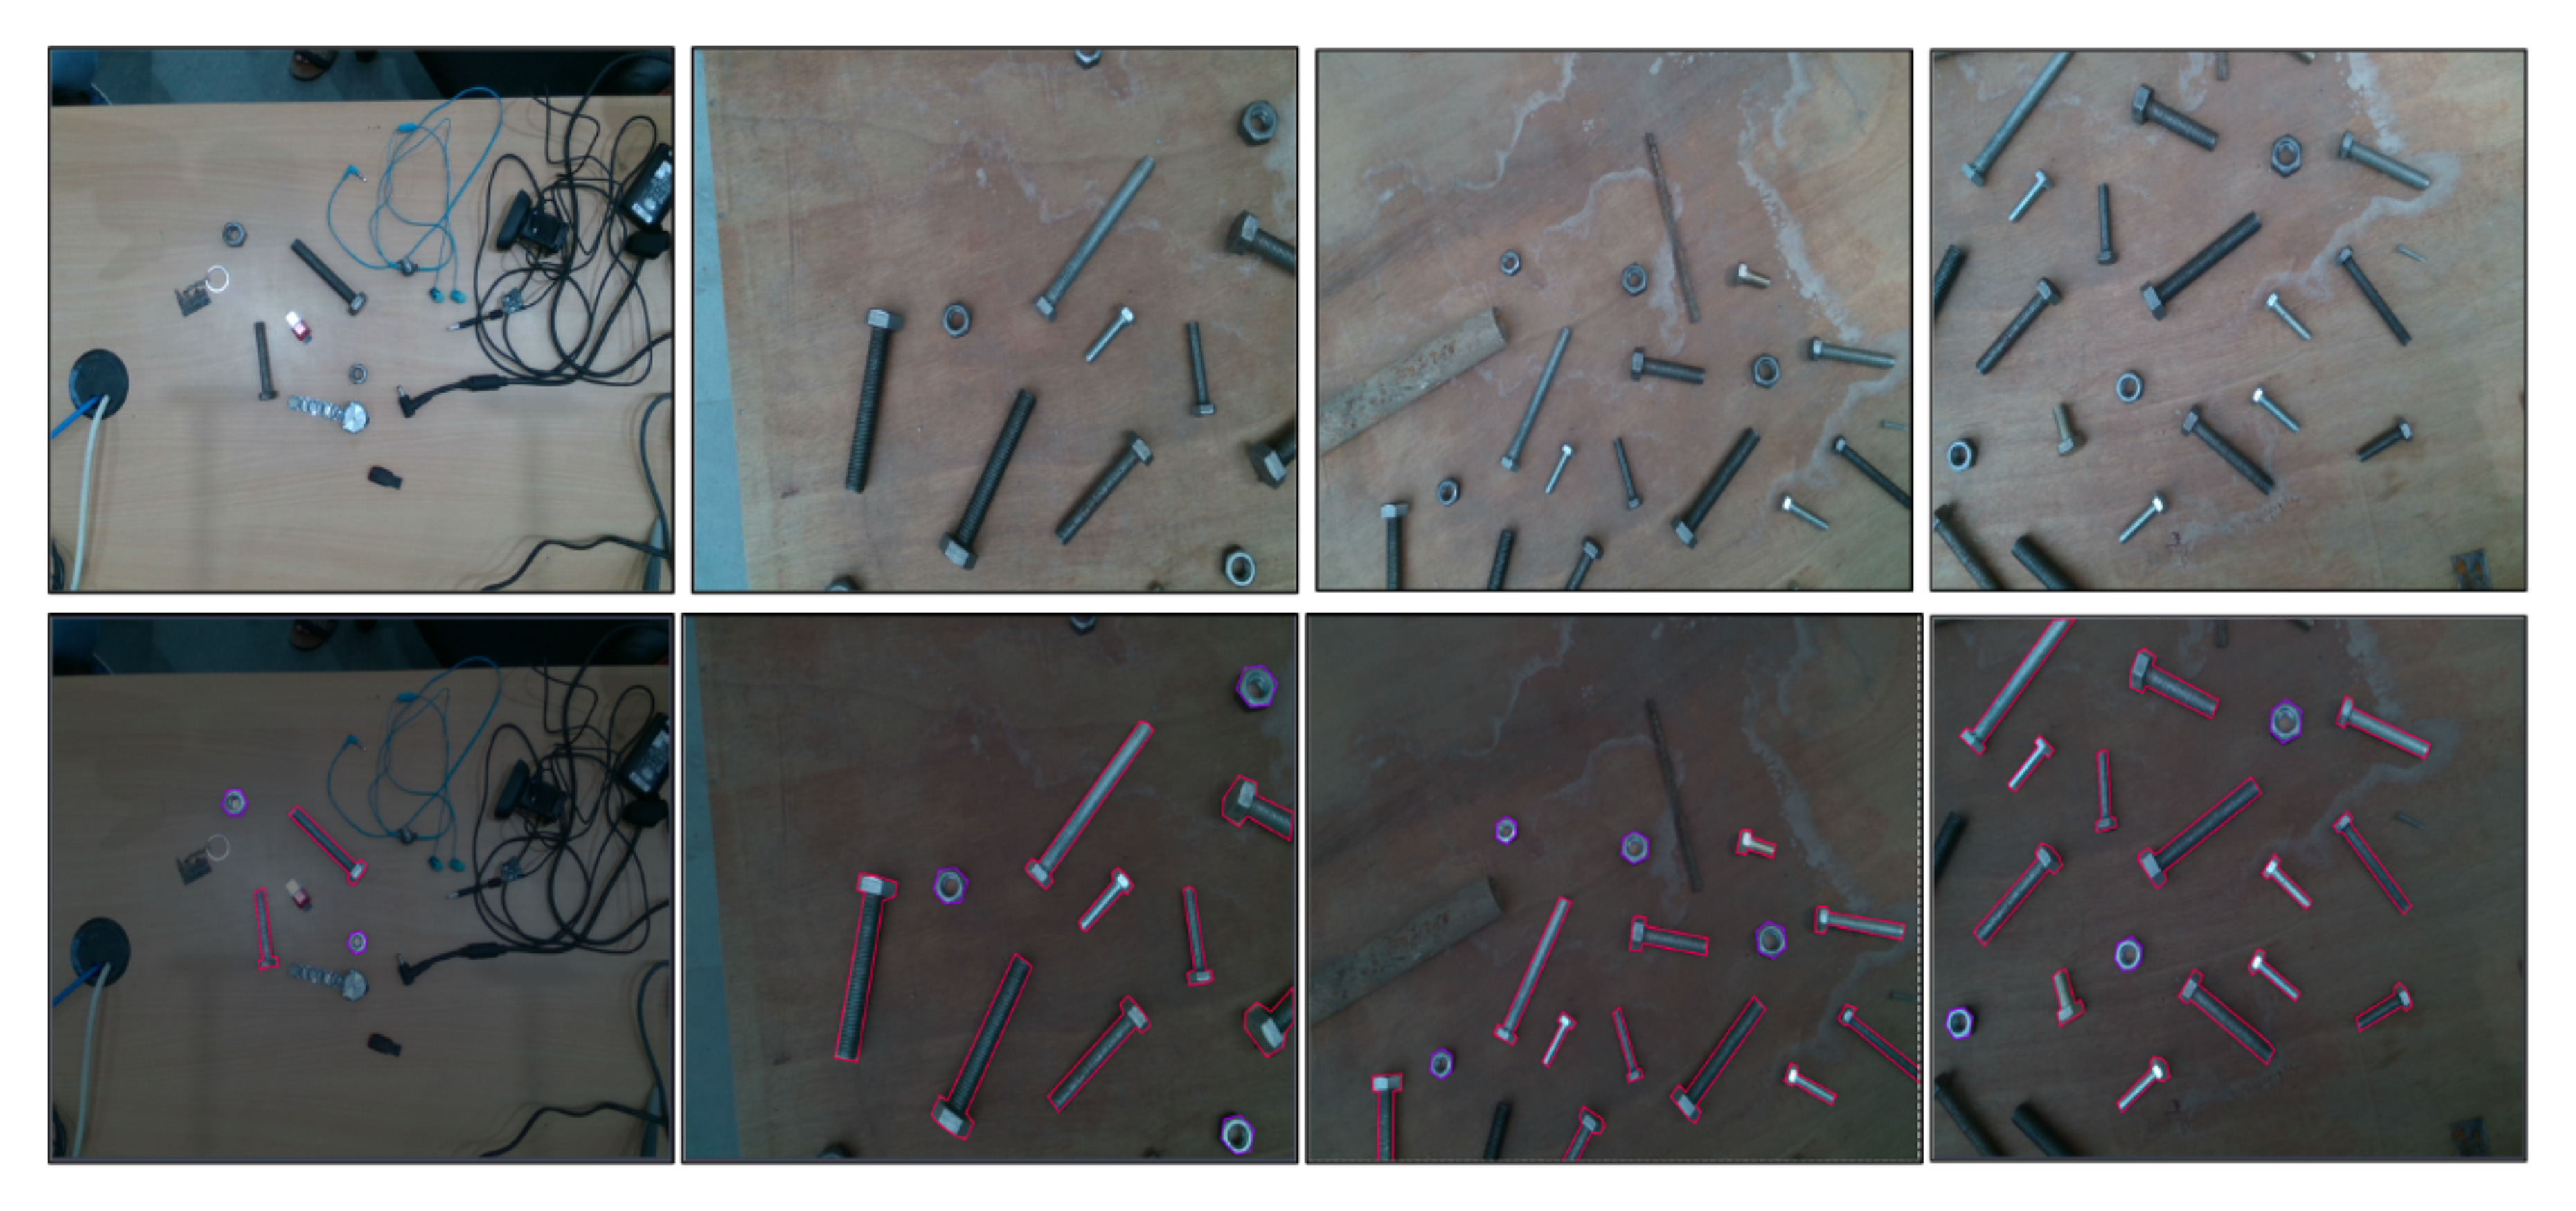
\includegraphics[width=0.85\linewidth]{Images/iapf/data_collection_labeling.jpg}
\caption{Data collection (top row) and labeling (bottom row) of nuts (blue border) and bolts (red
border) across varying backgrounds and lighting~\citep{surya2025iapf}.}
\label{fig:iapf_datacollection}
\end{figure}

\begin{figure}[htbp]
\centering
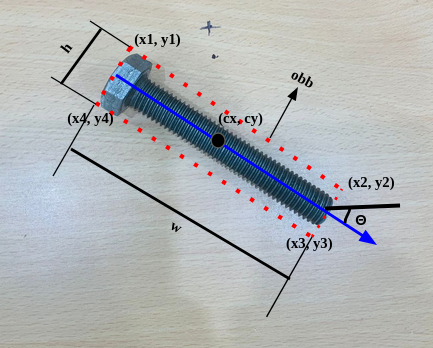
\includegraphics[width=0.5\linewidth]{Images/iapf/obb_detection.jpeg}
\caption{YOLOv8 oriented bounding box prediction around a detected bolt, giving centroid, head
width $h$, shank length $w$, and orientation $\theta$~\citep{surya2025iapf}.}
\label{fig:iapf_obb}
\end{figure}

%% ============================================================
\section{The Three-Way Force Equilibrium}\label{sec:iapf_forces}
%% ============================================================

iAPF retains the classical APF's reactive, gradient-like structure~\citep{khatib1986real} while
replacing each of its components: an exponential goal attraction, a continuous inverse-distance
inter-arm repulsion, and an exponential home-seeking force together form the three-way equilibrium
that gives the controller its name, stabilized by a fourth, velocity-dependent damping term. Let
$p_{ee}^\alpha$ denote the end-effector position of arm $\alpha \in \{L, R\}$ in the shared reference
frame $B_L$, and let $g$ denote a target's position from Section~\ref{sec:iapf_architecture}. The
goal attraction force grows exponentially with distance rather than linearly, giving sub-linear
growth near the goal for gentle convergence and super-linear growth far from it for a faster
approach, without gain scheduling:
\begin{equation}
\vec{f}_{\text{att}}(p_{ee}^\alpha, g) = k_a \left( e^{\lVert e \rVert} - 1 \right) \hat{e}, \qquad
e = g - p_{ee}^\alpha,\; \hat{e} = \frac{e}{\lVert e \rVert}.
\label{eq:iapf_attract}
\end{equation}
The inter-arm repulsive force uses a continuous inverse-distance law, smooth and non-zero at every
finite separation rather than switching on abruptly at a fixed cutoff radius as the classical
formulation does:
\begin{equation}
\vec{f}_{\text{rep}}(p_{ee}^L, p_{ee}^R) = k_r \frac{1}{d_{\min}^{\eta}}\, \hat{r}, \qquad
\hat{r} = \frac{p_{ee}^R - p_{ee}^L}{\lVert p_{ee}^R - p_{ee}^L \rVert},
\label{eq:iapf_repel}
\end{equation}
where $d_{\min} = \min(D_{\text{inter}})$ is exactly the minimum inter-arm link distance of
Equation~\eqref{eq:dm_interarm} from Chapter~\ref{chap:distance}, computed once per control cycle
from the closed-form line-segment distances of Section~\ref{sec:dm_distance}. The home-seeking
force is the novel addition beyond the classical two-force formulation: it uses the same exponential
form as attraction to draw an idle or displaced arm back toward a predefined safe position
$h_\alpha$,
\begin{equation}
\vec{f}_{\text{home}}(p_{ee}^\alpha, h_\alpha) = k_h \left( e^{\lVert e_h \rVert} - 1 \right) \hat{e}_h,
\qquad e_h = h_\alpha - p_{ee}^\alpha,
\label{eq:iapf_home}
\end{equation}
and, as demonstrated in Section~\ref{sec:iapf_validation}, is what prevents the oscillation and
excessive arm extension that the two-force formulation alone exhibits near simultaneous goal
conflicts. Velocity damping opposes the arm's own motion,
\begin{equation}
\vec{f}_{\text{damp}}(\vec{v}_\alpha) = -k_d\, \vec{v}_\alpha,
\label{eq:iapf_damp}
\end{equation}
and the resultant force combines all four components,
\begin{equation}
\vec{f}_{\text{resultant}} = \vec{f}_{\text{att}} + \vec{f}_{\text{rep}} + \vec{f}_{\text{home}}
- k_d\, \vec{v},
\label{eq:iapf_resultant}
\end{equation}
with $k_a, k_r, k_h, k_d > 0$ gain constants and $\eta$ the repulsion decay exponent.

%% ============================================================
\section{Velocity Generation and Orientation Control}\label{sec:iapf_velocity}
%% ============================================================

The resultant force of Equation~\eqref{eq:iapf_resultant} is converted directly to a commanded
Cartesian velocity by a single scaling factor,
\begin{equation}
\vec{v}_k = \frac{\left(\vec{f}_{\text{resultant}}\right)_k}{s}, \qquad k \in \{L, R\},
\label{eq:iapf_velocity}
\end{equation}
so that the manipulator's kinematic state evolves as $\dot{x} = v = k_v\, \vec{f}_{\text{resultant}}(x)$
for end-effector position $x \in \mathbb{R}^3$ and scalar $k_v = 1/s$, the closed-loop system whose
behaviour Section~\ref{sec:iapf_validation} validates experimentally.

Orientation is controlled in parallel. The current end-effector orientation
$\boldsymbol{\theta}_c = [\theta_{cx}, \theta_{cy}, \theta_{cz}] \in SO(3)$ comes from real-time
forward kinematics, and the desired orientation $\boldsymbol{\theta}_d = [\theta_{dx}, \theta_{dy}, \theta_{dz}]$
from vision, using the gripper yaw of Equation~\eqref{eq:iapf_gripperangle} for $\theta_{dz}$. Both
are assembled into rotation matrices $R(\boldsymbol{\theta}) = R_z(\theta_z) R_y(\theta_y) R_x(\theta_x)$,
and the orientation error rotation matrix is
\begin{equation}
R_e = R_d R_c^{-1} \in SO(3),
\label{eq:iapf_orierror}
\end{equation}
expressed in axis-angle form, error angle $\theta \in \mathbb{R}$ about axis
$\mathbf{k} = [k_x, k_y, k_z]$. The PD control law for angular velocity is
\begin{equation}
\vec{\omega} = K_p \cdot \theta \cdot \mathbf{k} + K_d \cdot \frac{d}{dt}(\theta \cdot \mathbf{k}),
\label{eq:iapf_angular}
\end{equation}
with $K_p, K_d \in \mathbb{R}^{3 \times 3}$ diagonal gain matrices. Equations~\eqref{eq:iapf_velocity}
and~\eqref{eq:iapf_angular} together are the hybrid linear-angular twist controller: iAPF-derived
linear velocity coupled to independent PD-regulated angular velocity, both computed in the shared
reference frame and rotated into the right arm's own frame by $R^{B_L}_{B_R}$ before being sent, as
in Equation~\eqref{eq:sv_thetae}'s counterpart for the resolved-rate controller of
Chapter~\ref{chap:shared_vision}.

%% ============================================================
\section{Priority-Based Coordination: the Original Fixed Assignment}\label{sec:iapf_priority}
%% ============================================================

In its original validation, iAPF assigns objects to arms by a fixed convention, every detected nut
to the left arm and every detected bolt to the right, illustrated in
Figure~\ref{fig:iapf_setup}. This is precisely the limitation identified as gap G5: an object of the
"wrong" type for its nearest arm cannot be picked up by that arm regardless of proximity. What the
original paper does address is the coordination problem this fixed assignment still leaves open, two
arms independently converging on the shared workspace can still create a near-goal conflict, which
is resolved by a priority-lock state machine (Figure~\ref{fig:iapf_statemachine}).

\begin{figure}[htbp]
\centering
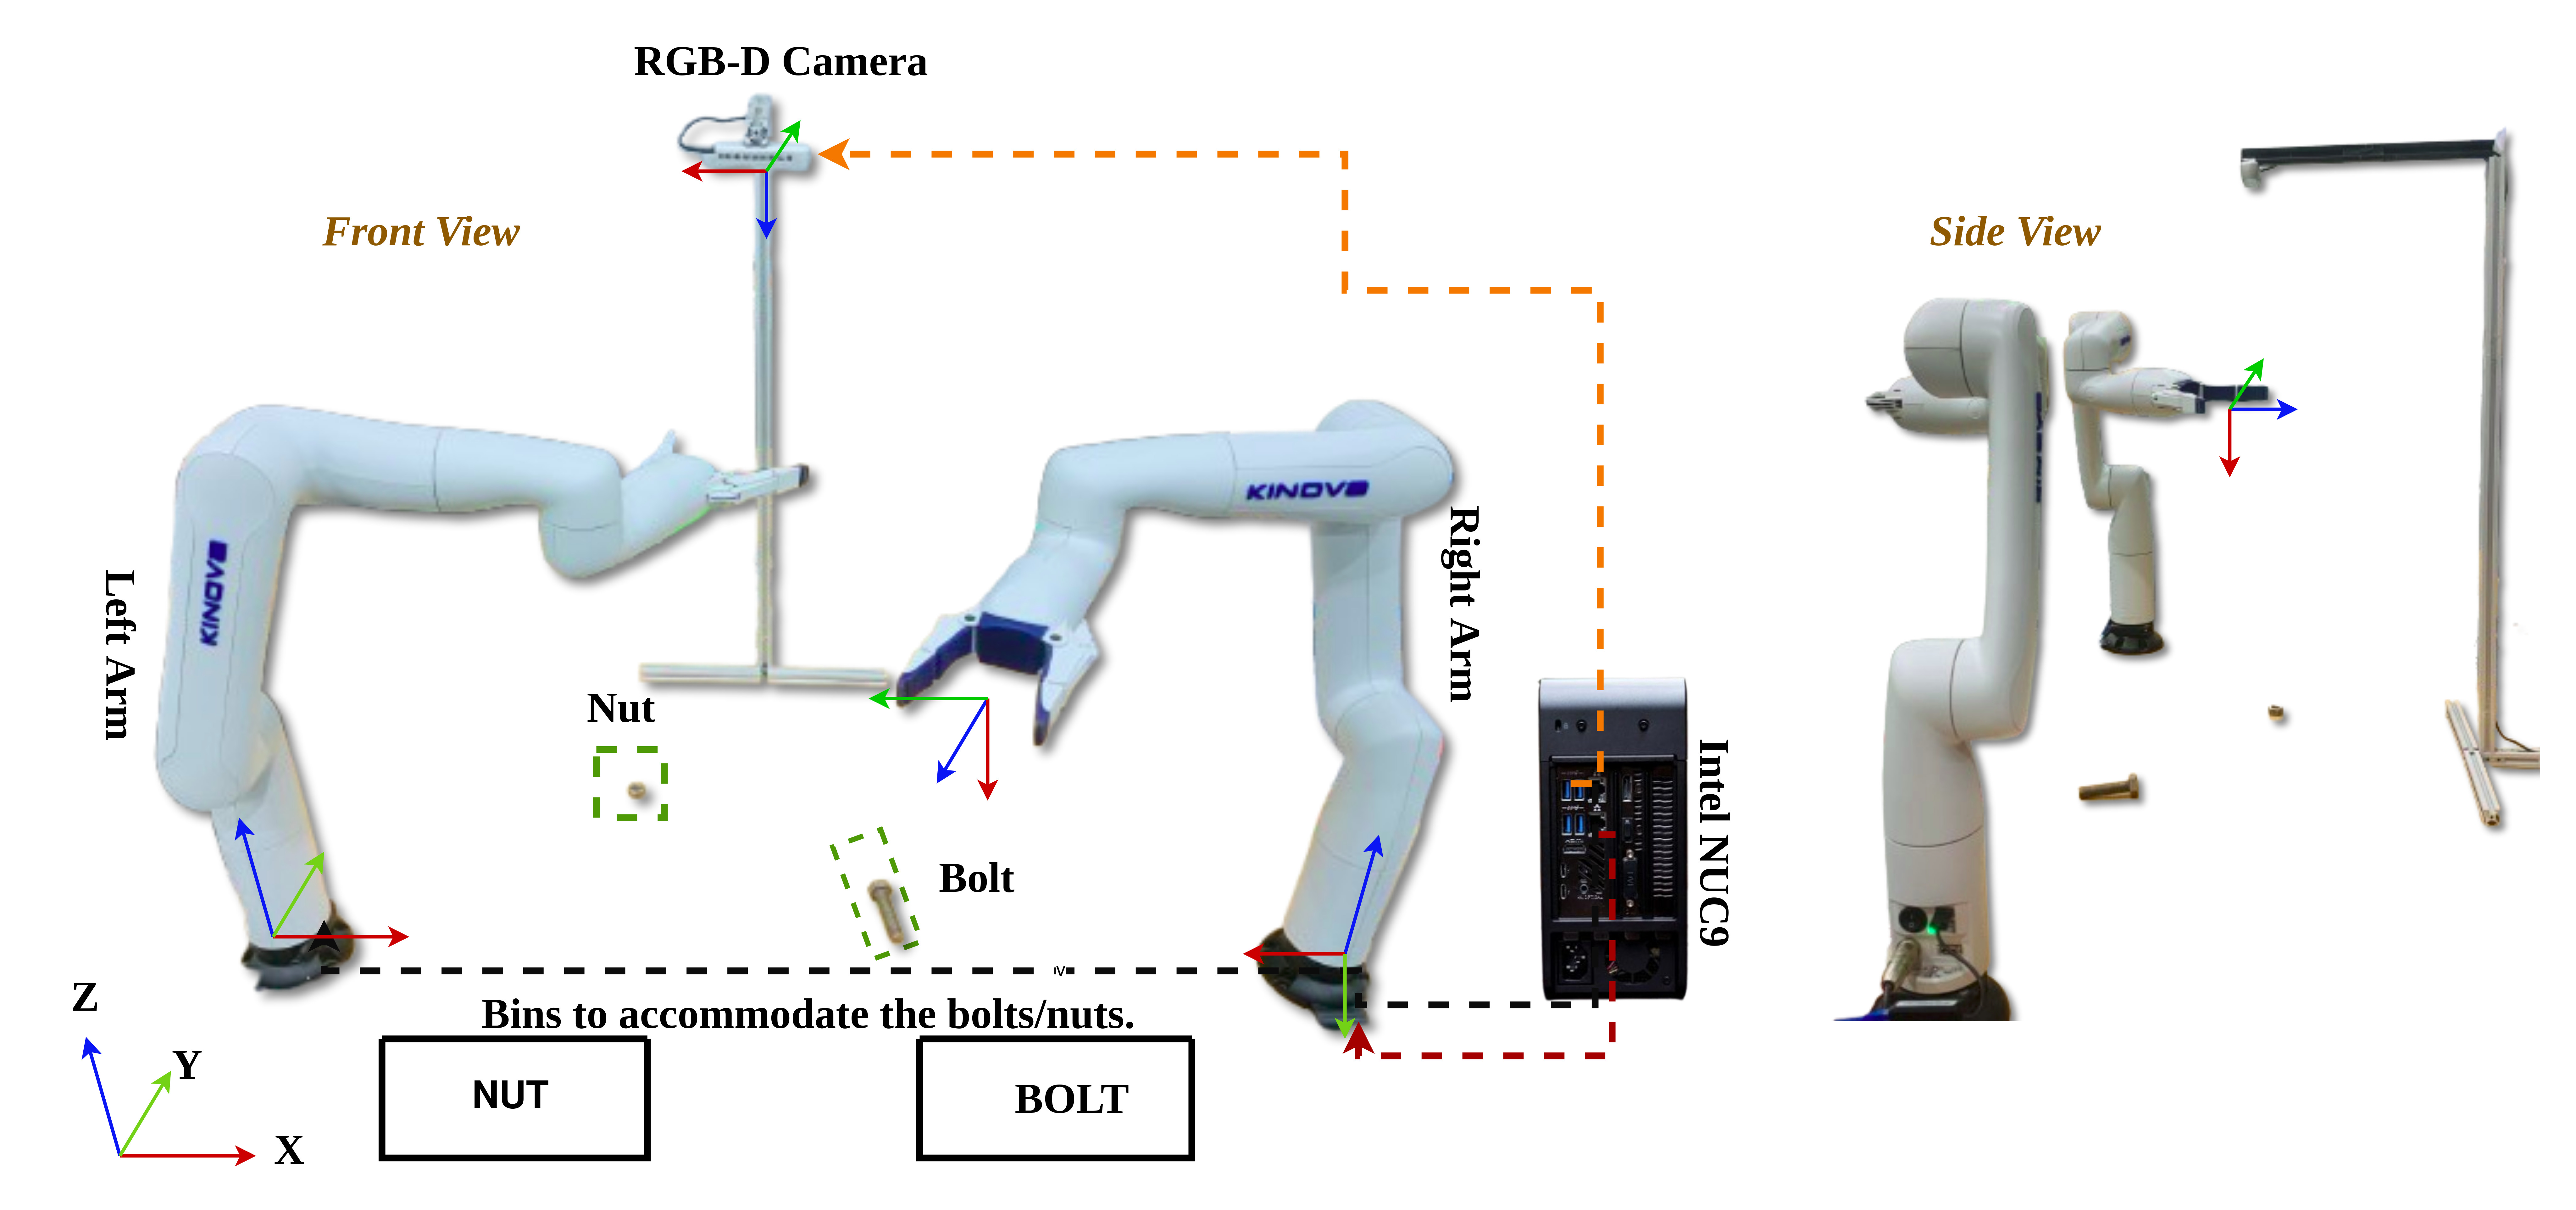
\includegraphics[width=0.85\linewidth]{Images/iapf/experimental_setup.jpg}
\caption{Experimental setup for the original iAPF validation, with the fixed nut-left/bolt-right
assignment~\citep{surya2025iapf}.}
\label{fig:iapf_setup}
\end{figure}

Each arm cycles through IDLE, PICK, PICK\_LOCK, GRIP, PLACE, PLACE\_LOCK, UNGRIP, and DONE states.
PICK\_LOCK, GRIP, PLACE\_LOCK, and UNGRIP are the critical states, in which precision matters more
than collision avoidance: on entering one of them, the task-adaptive weights of
Equation~\eqref{eq:iapf_resultant}'s implicit coefficients are set so that $\vec{f}_{\text{rep}}$
and $\vec{f}_{\text{home}}$ are switched off entirely, leaving only goal attraction and damping to
drive the final approach undisturbed by the other arm's motion. Outside the critical states, both
forces remain active. When both arms are simultaneously in PICK, or simultaneously in PLACE, a
priority mechanism compares their remaining distance to target and locks the closer arm into its
respective critical state first, holding the other arm in the full four-force regime until the
locked arm completes its critical maneuver (Figure~\ref{fig:iapf_prioritylock}).

\begin{figure}[htbp]
\centering
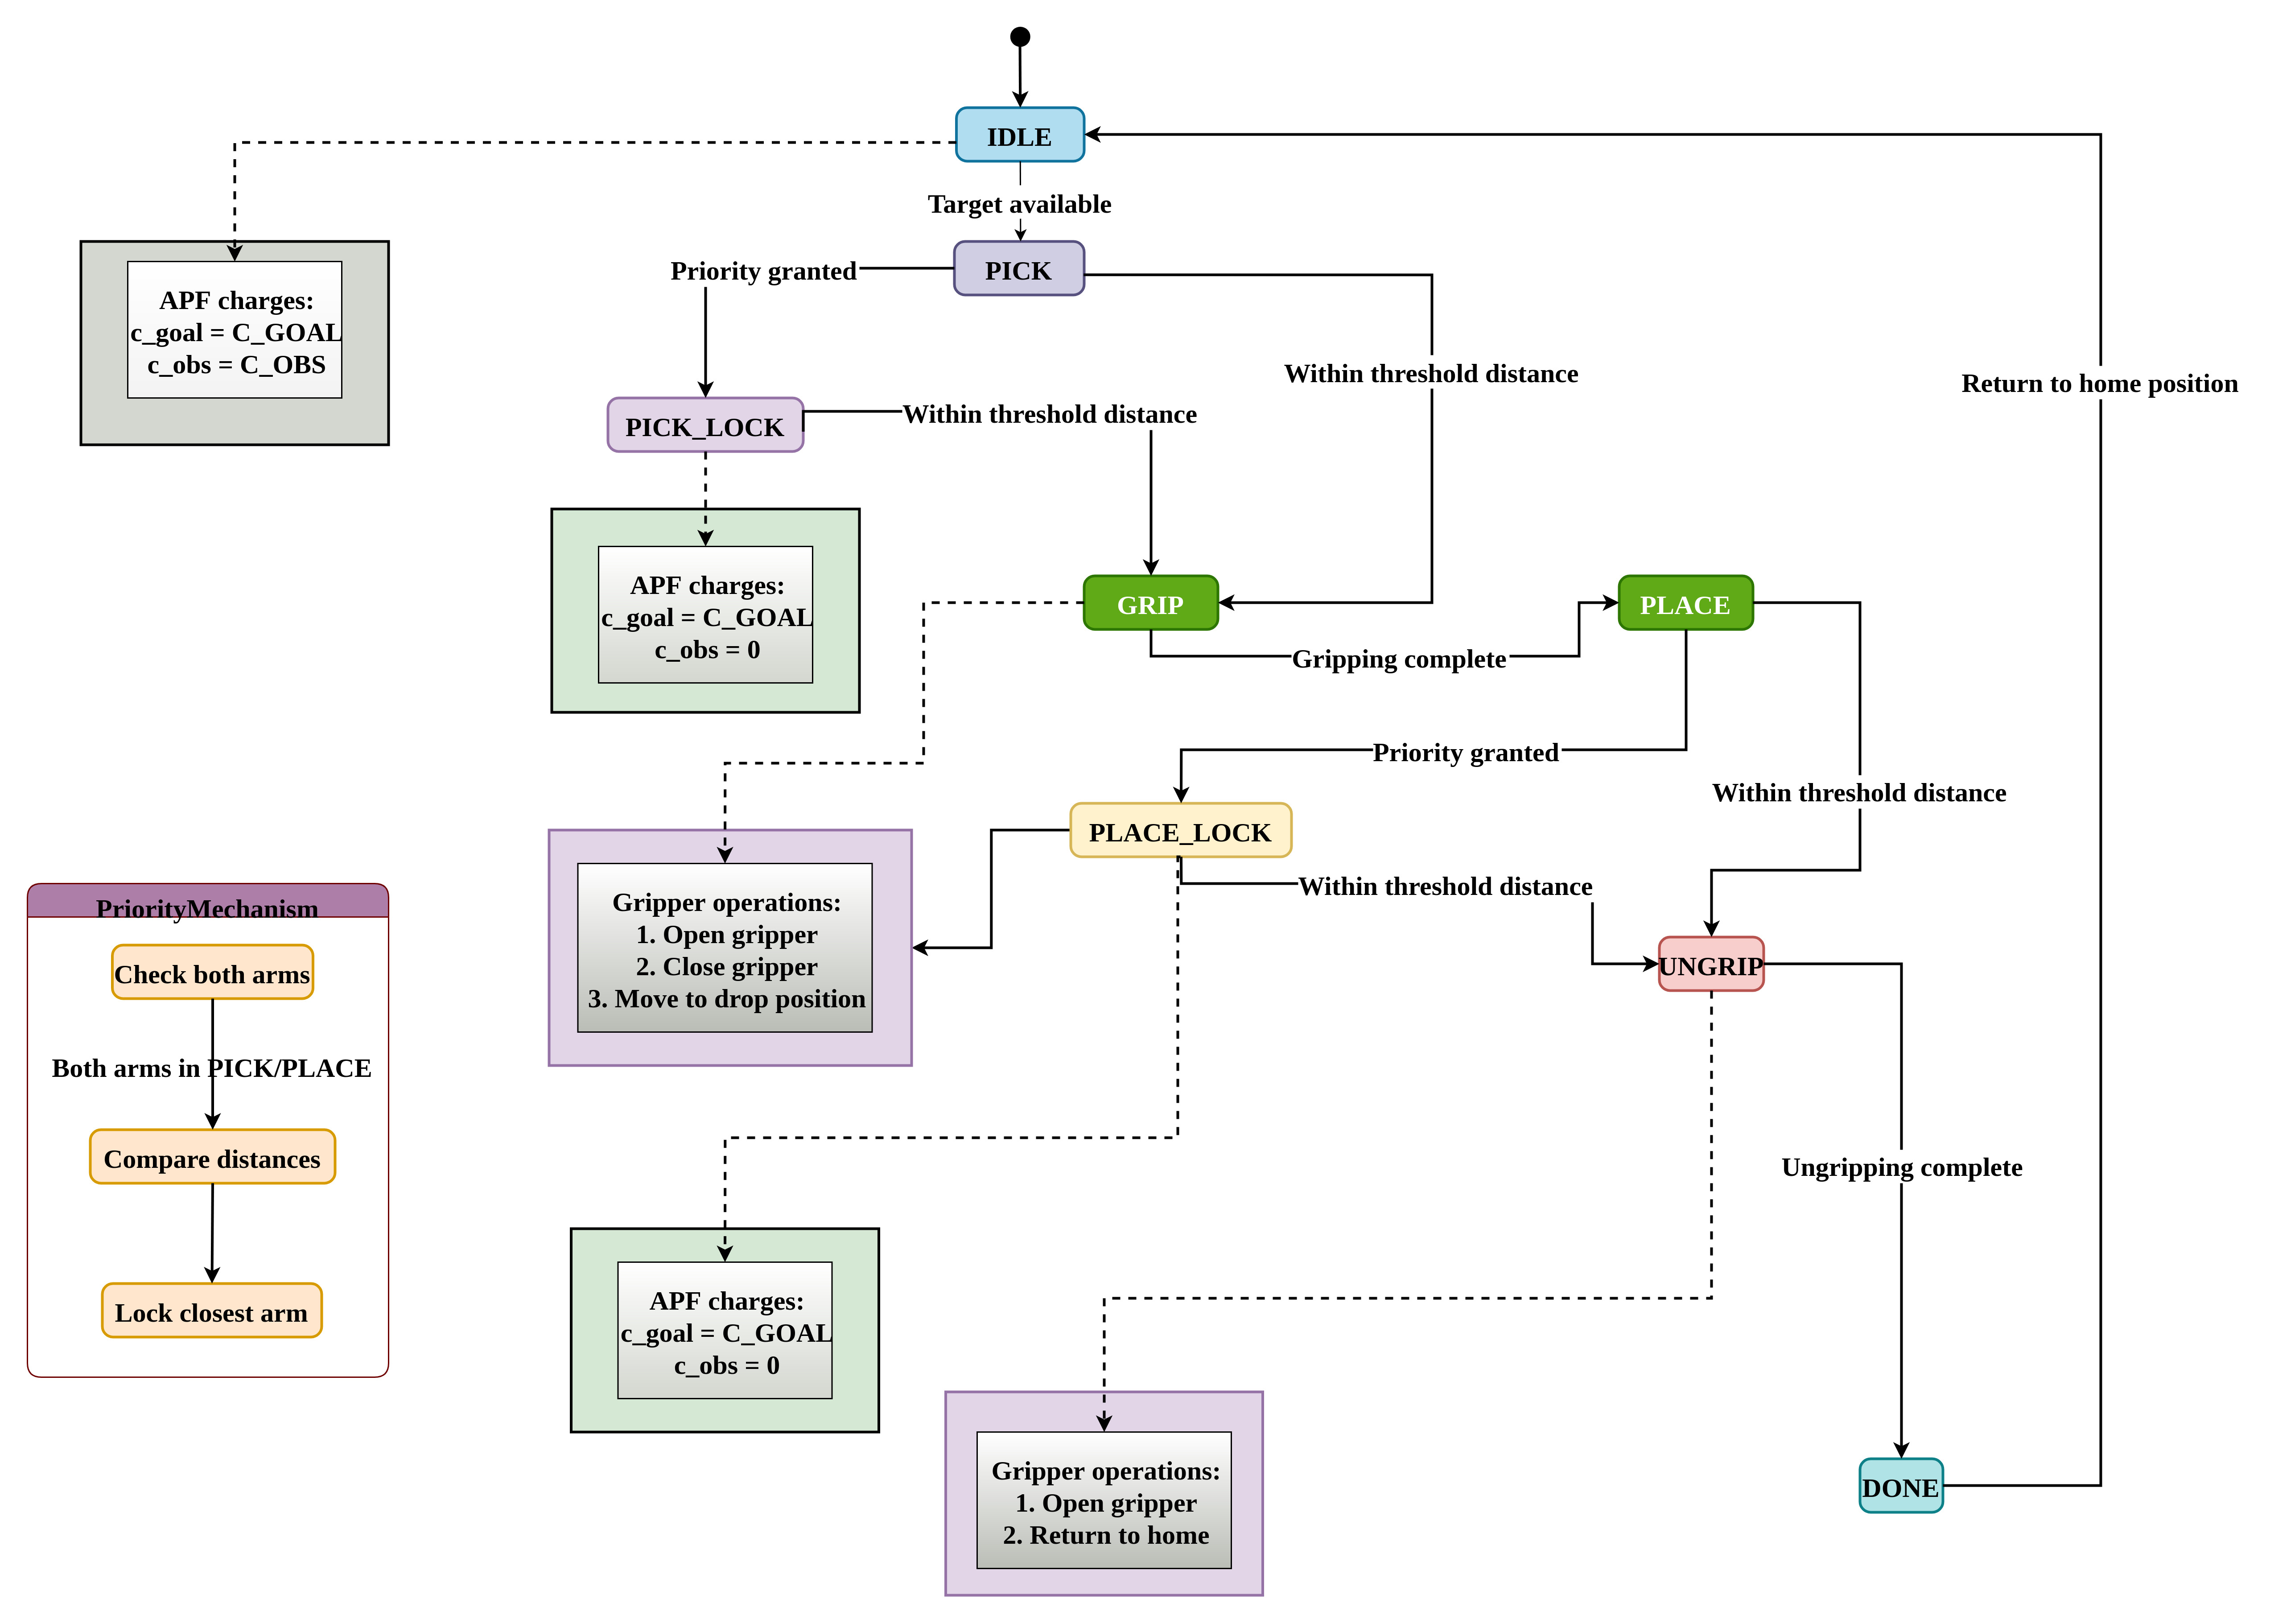
\includegraphics[width=0.85\linewidth]{Images/iapf/state_machine.jpg}
\caption{Overall per-arm state machine for the original iAPF pick-and-place sequence: IDLE $\to$
PICK $\to$ PICK\_LOCK $\to$ GRIP $\to$ PLACE $\to$ PLACE\_LOCK $\to$ UNGRIP $\to$ DONE, with
force-field coefficients $(c_{\text{goal}}, c_{\text{obs}})$ annotated at each transition, and the
priority mechanism summarized at bottom left~\citep{surya2025iapf}.}
\label{fig:iapf_statemachine}
\end{figure}

\begin{figure}[htbp]
\centering
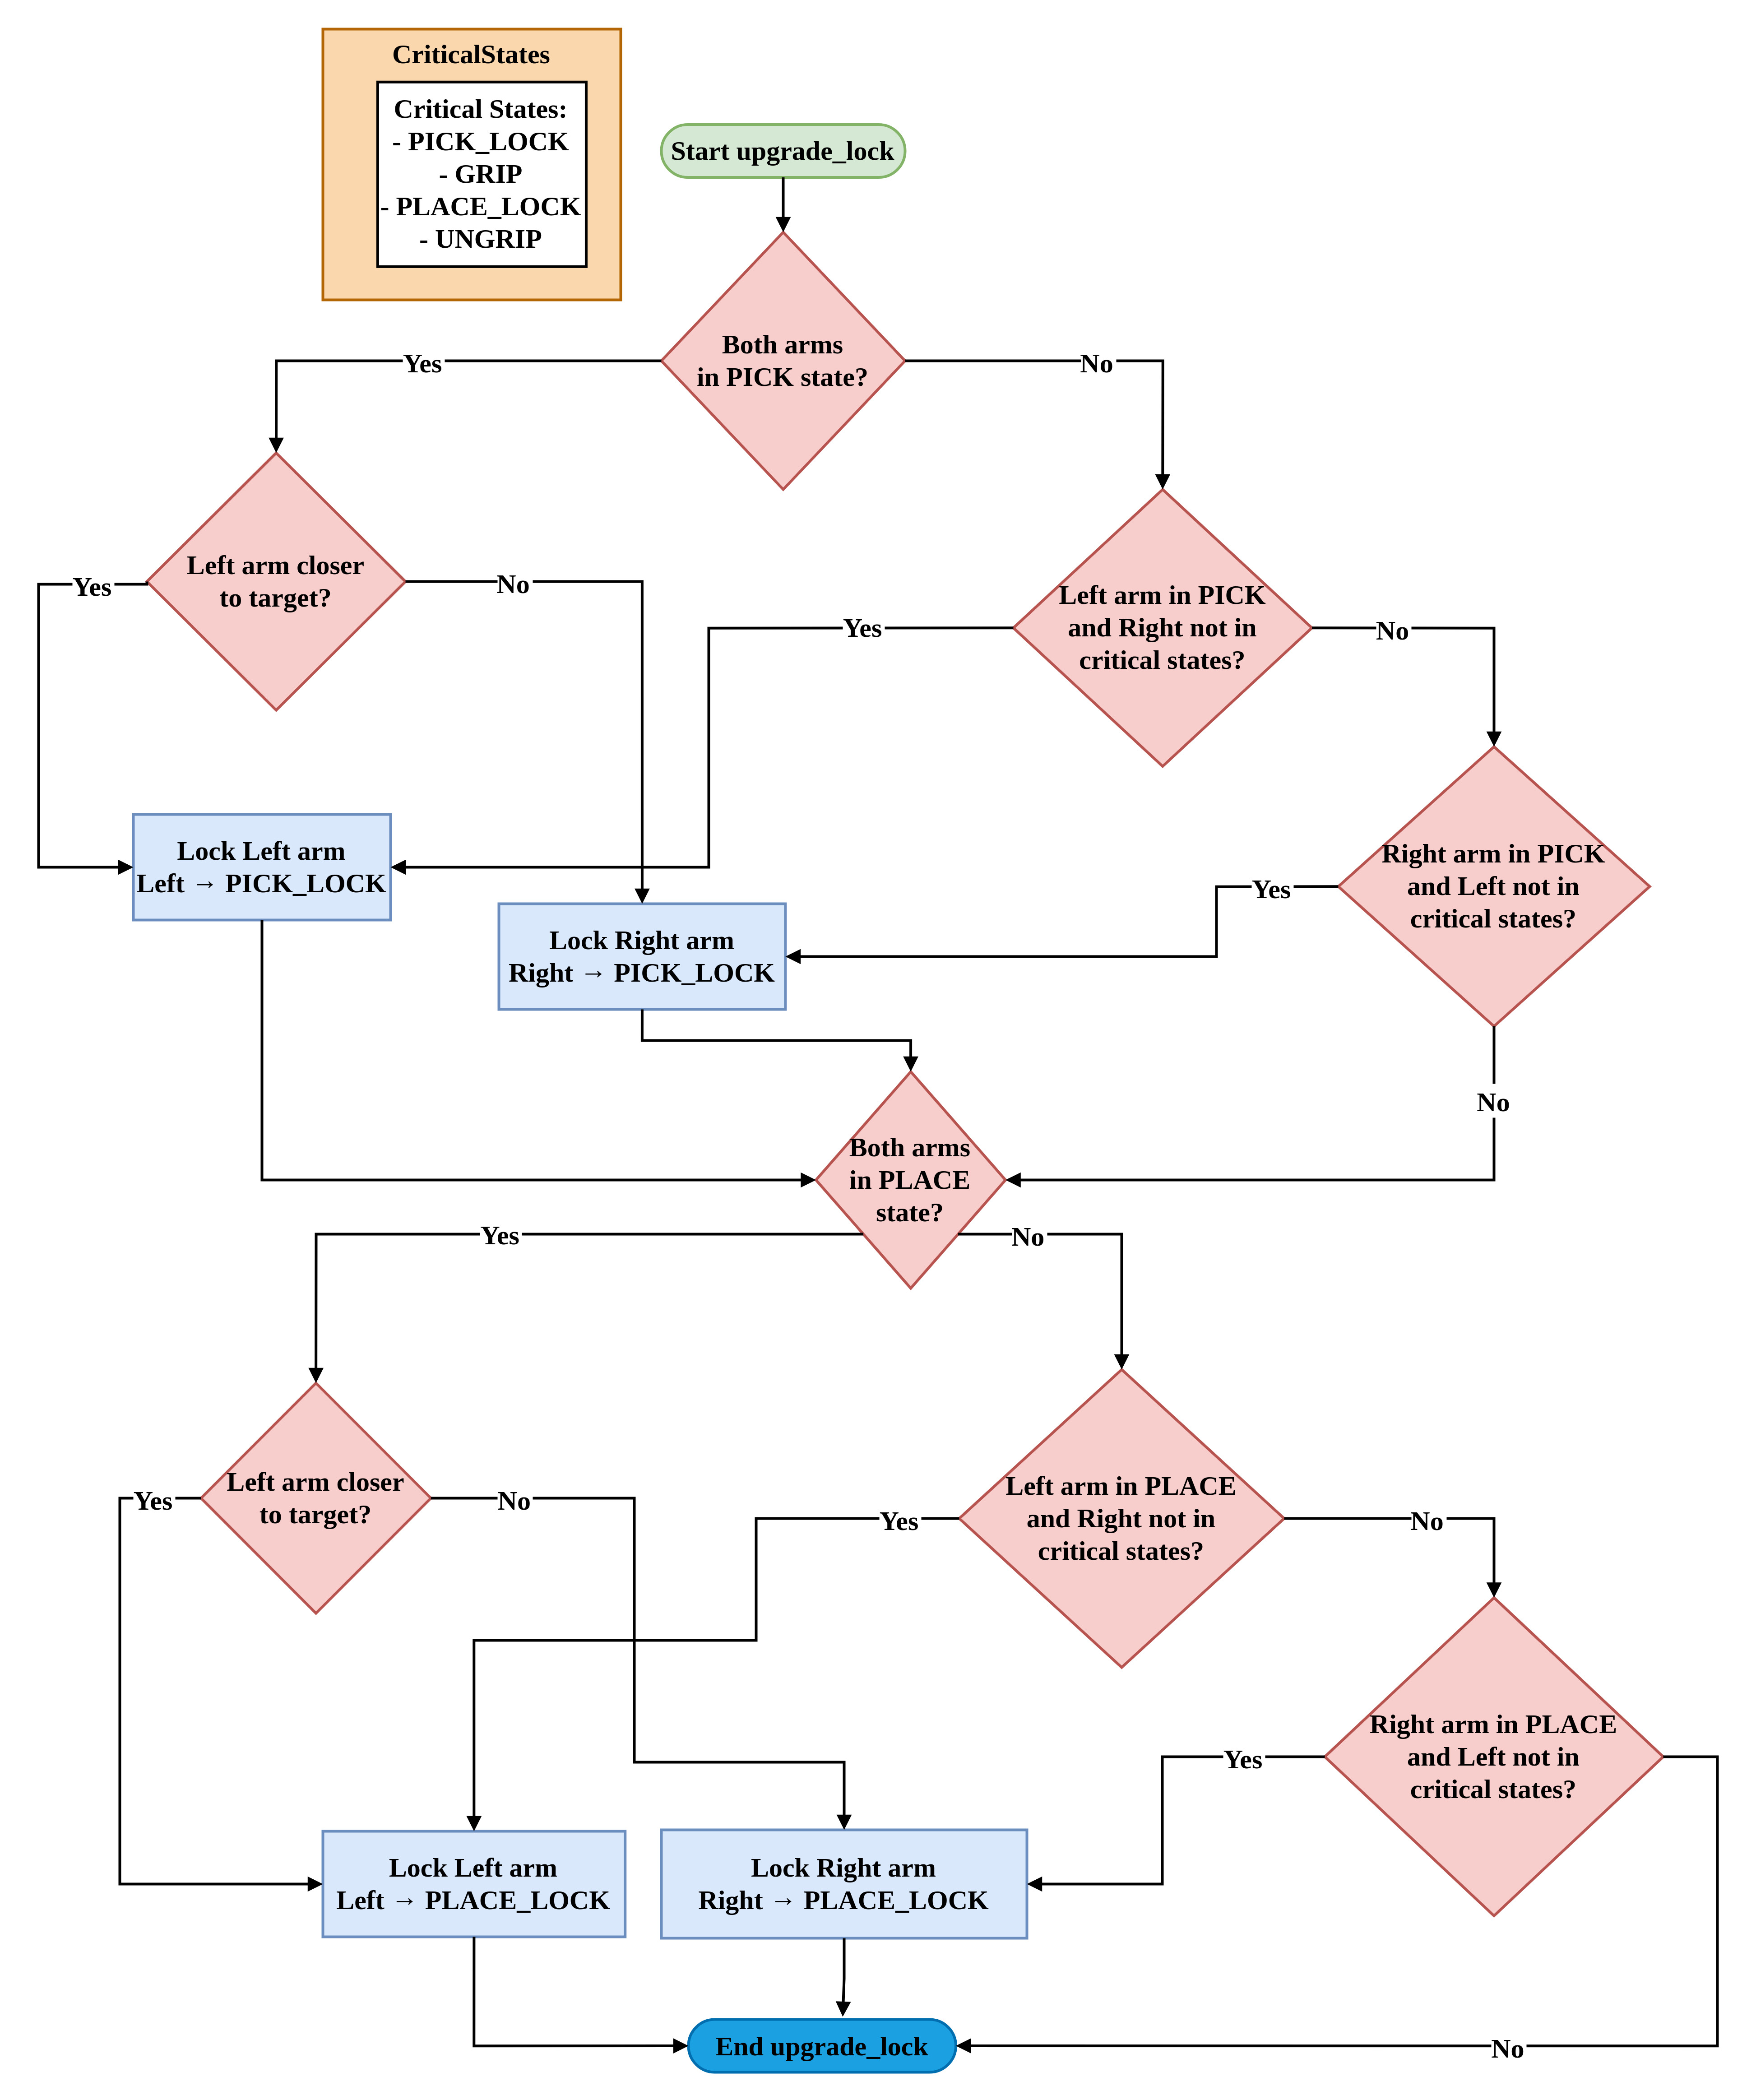
\includegraphics[width=0.75\linewidth]{Images/iapf/priority_lock.jpg}
\caption{Priority-lock decision flow: when both arms are in PICK (or both in PLACE), the arm closer
to its target is locked into the critical state first; the other arm remains in the full four-force
regime until the lock is released~\citep{surya2025iapf}.}
\label{fig:iapf_prioritylock}
\end{figure}

%% ============================================================
\section{Empirical Validation: the Necessity of the Home-Seeking Force}\label{sec:iapf_validation}
%% ============================================================

The three-way force equilibrium of Section~\ref{sec:iapf_forces} and the hybrid twist controller of
Section~\ref{sec:iapf_velocity} are validated directly on hardware rather than through a closed-form
stability proof: the resultant force of Equation~\eqref{eq:iapf_resultant} is the commanded velocity
itself, so its behaviour is exactly what repeated dual-arm trials show. The home-seeking term's
practical necessity is demonstrated experimentally by comparing the full three-way equilibrium
against the classical two-way (attraction and repulsion only) formulation under an identical
near-goal conflict.

\begin{figure}[htbp]
\centering
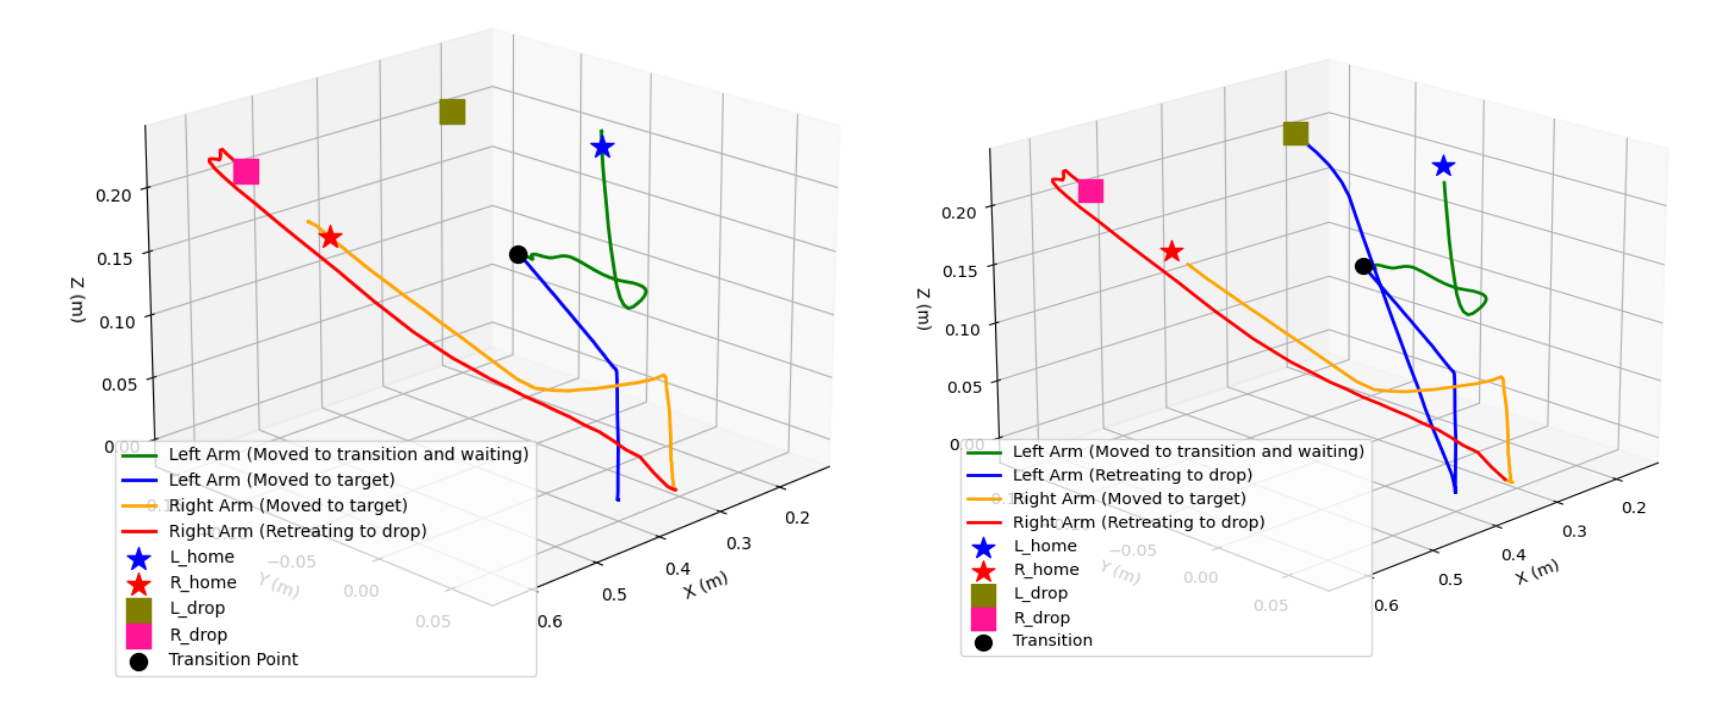
\includegraphics[width=0.85\linewidth]{Images/iapf/trajectories_with_home.png}
\caption{Dual-arm end-effector trajectories with the home-seeking force active (three-way
equilibrium): both arms initiate from home, the right arm reaches its target first under distance
priority and retreats to its drop point, and the left arm, holding at the transition point in the
meantime, then proceeds~\citep{surya2025iapf}.}
\label{fig:iapf_traj_with}
\end{figure}

\begin{figure}[htbp]
\centering
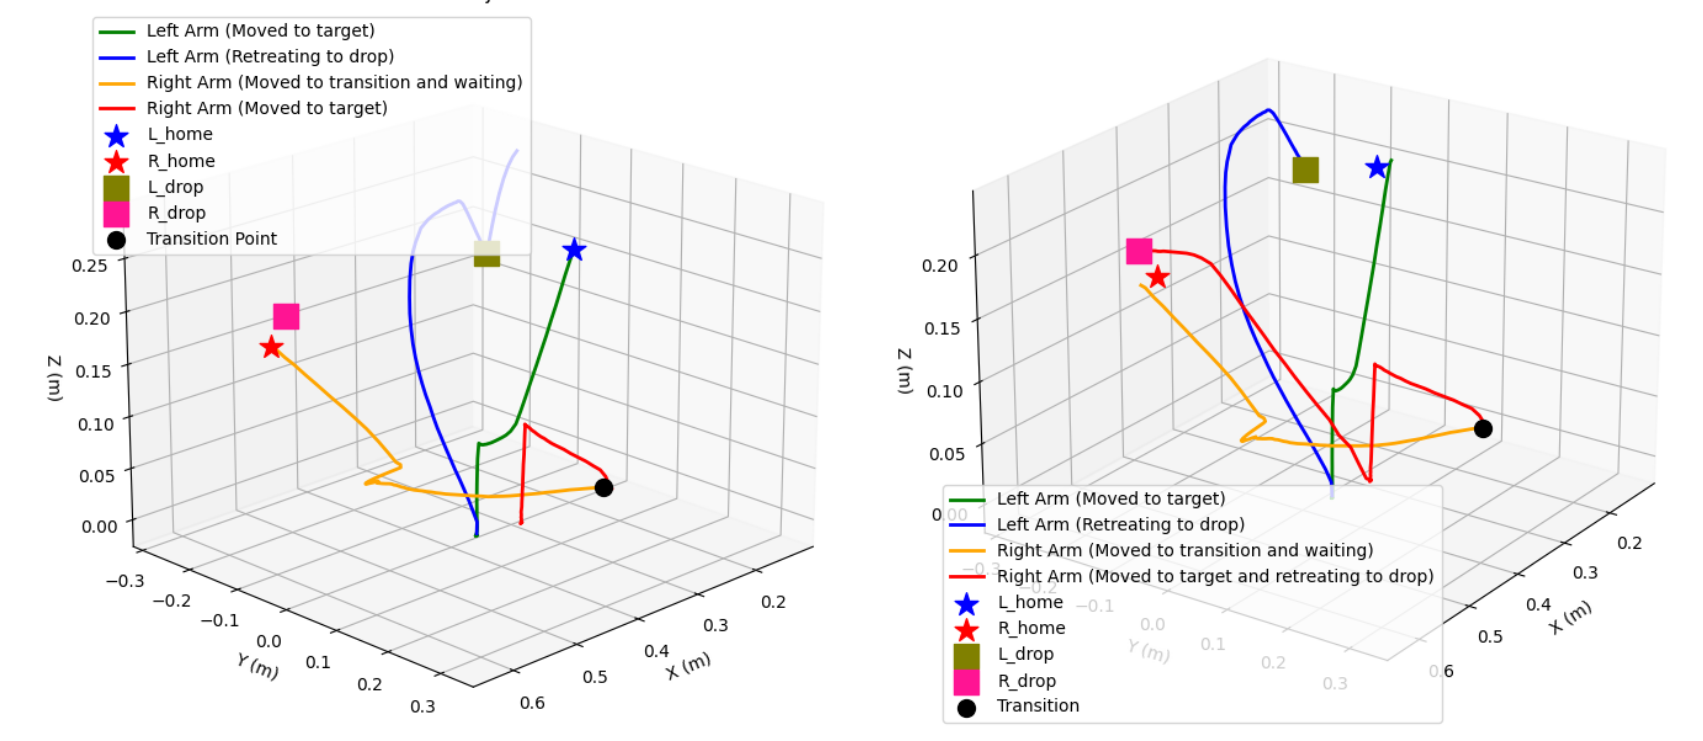
\includegraphics[width=0.85\linewidth]{Images/iapf/trajectories_without_home.png}
\caption{Dual-arm end-effector trajectories without the home-seeking force (two-way equilibrium),
the same conflict, showing wider sweeping motions and more visible path curvature during the
approach~\citep{surya2025iapf}.}
\label{fig:iapf_traj_without}
\end{figure}

Figure~\ref{fig:iapf_traj_with} and Figure~\ref{fig:iapf_traj_without} show the resulting
end-effector paths: without home-seeking, the two arms' attractive forces dominate as they approach
their respective goals while the inter-arm distance decreases, producing a sudden spike in repulsive
force that the two-way formulation has no mechanism to absorb, causing wide, oscillatory sweeps and
occasional over-extension toward kinematic singularities. With home-seeking active, the same
conflict instead produces the clean, bounded transition of
Figure~\ref{fig:iapf_traj_with}, consistent with the stability argument above: the home potential
gives the lower-priority arm a well-defined attractor to retreat toward rather than leaving it
subject only to the (now locally dominant) repulsive term.

\begin{figure}[htbp]
\centering
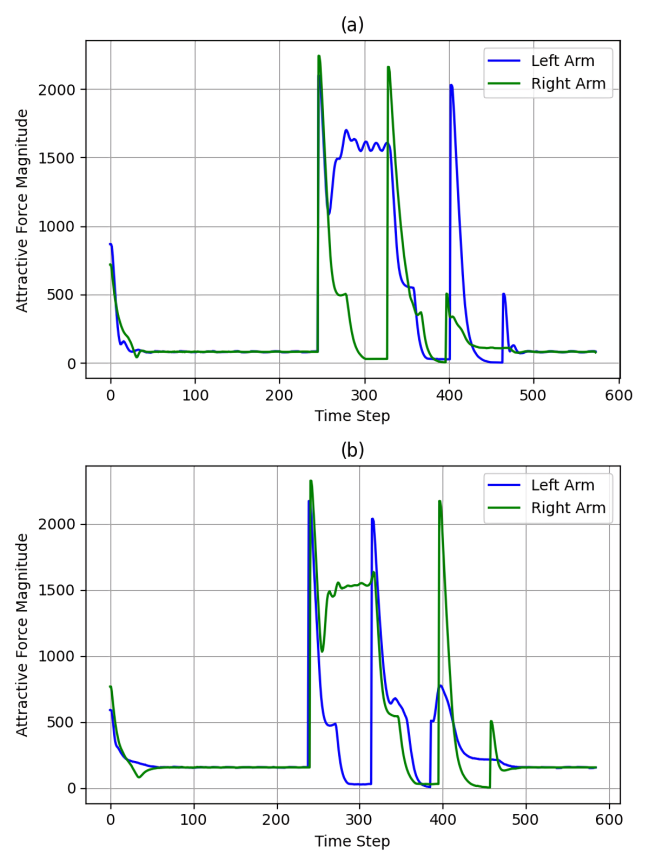
\includegraphics[width=0.7\linewidth]{Images/iapf/attractive_force_convergence.jpg}
\caption{Convergence of attractive forces for both arms, (a) with and (b) without the exponential
home-seeking force. With home-seeking, both arms show controlled convergence to a low baseline
before target detection and a single dominant peak per arm during the priority handoff; without it,
the baseline is held less tightly and both arms show competing attractive spikes around the
transition~\citep{surya2025iapf}.}
\label{fig:iapf_attforce}
\end{figure}

\begin{figure}[htbp]
\centering
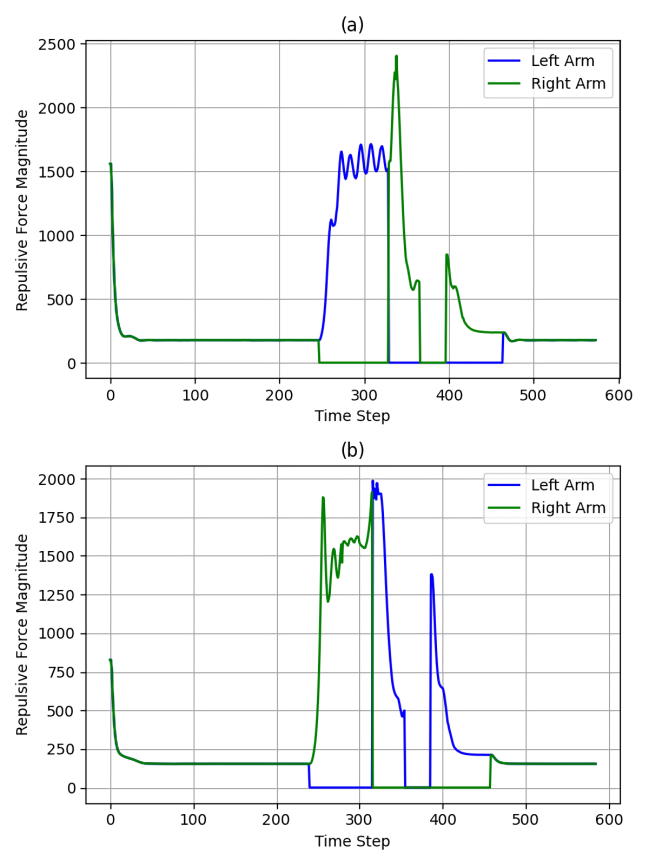
\includegraphics[width=0.7\linewidth]{Images/iapf/repulsive_force_convergence.jpg}
\caption{Convergence of repulsive forces for both arms, (a) with and (b) without the exponential
home-seeking force, showing the same qualitative contrast as
Figure~\ref{fig:iapf_attforce}~\citep{surya2025iapf}.}
\label{fig:iapf_repforce}
\end{figure}

\begin{figure}[htbp]
\centering
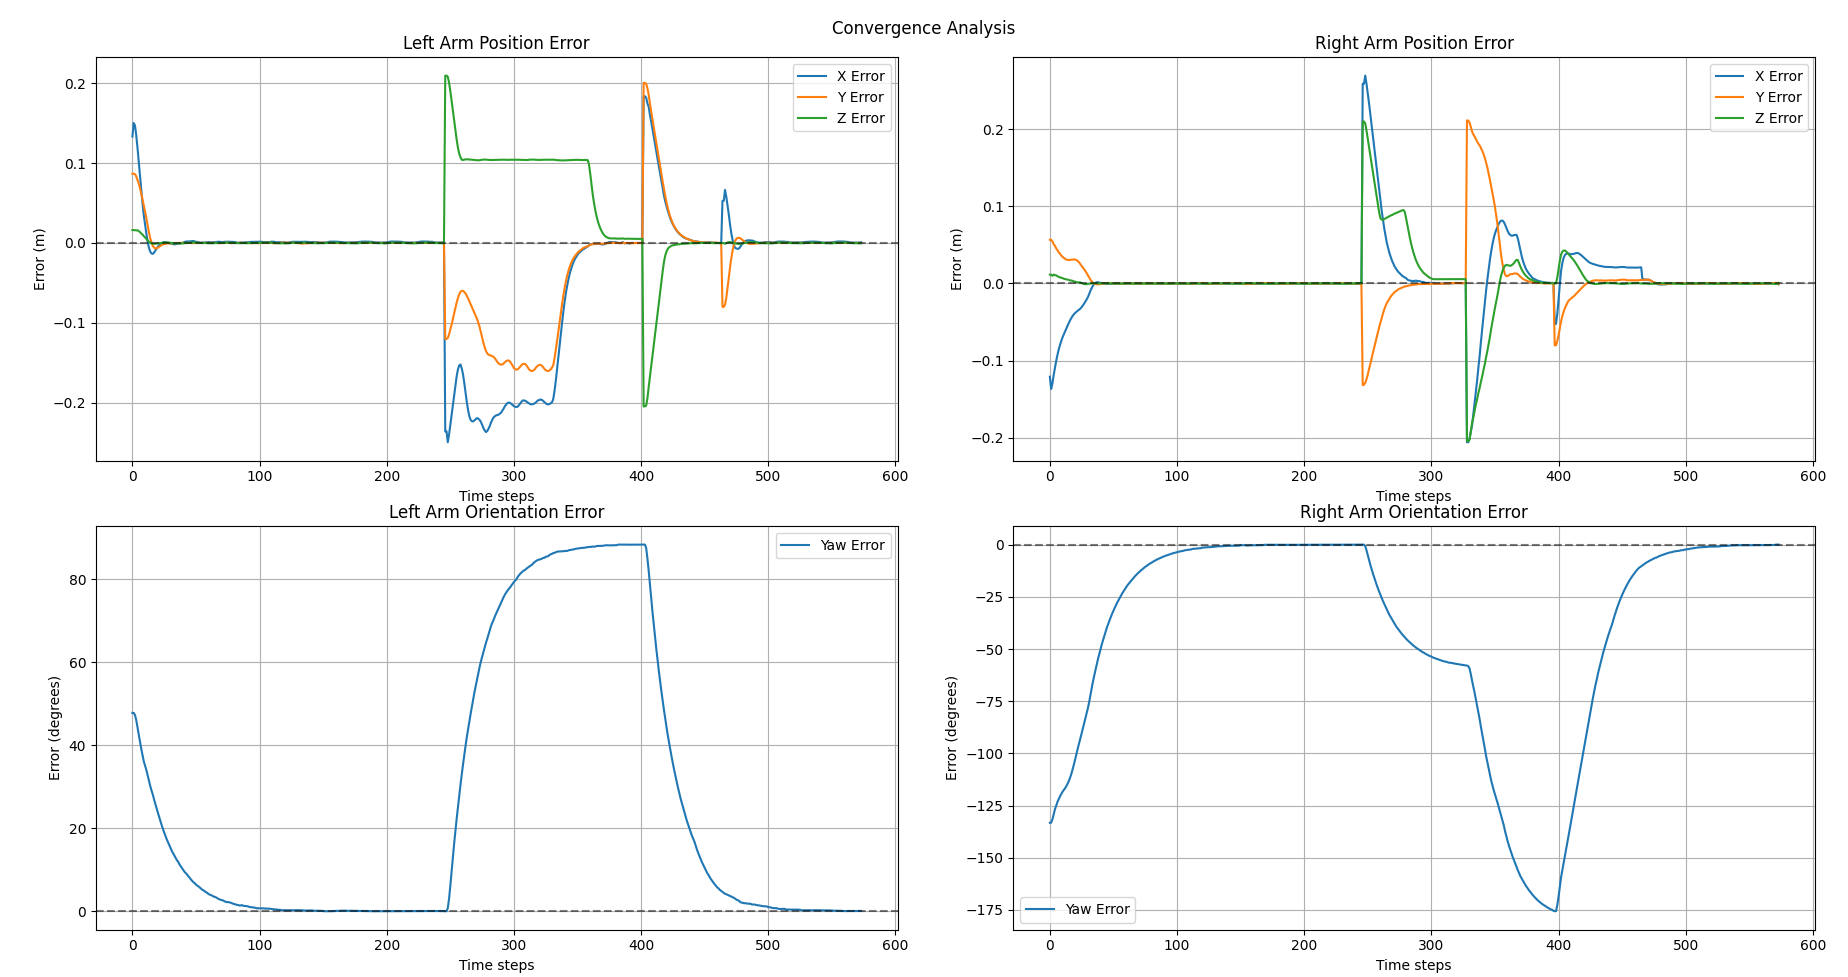
\includegraphics[width=0.9\linewidth]{Images/iapf/convergence_with_home.jpg}
\caption{Position and orientation error convergence with home-seeking active: a single clean
transient at each waypoint, position governed by the iAPF force law and orientation by the
independent PD loop of Equation~\eqref{eq:iapf_angular}~\citep{surya2025iapf}.}
\label{fig:iapf_error_with}
\end{figure}

\begin{figure}[htbp]
\centering
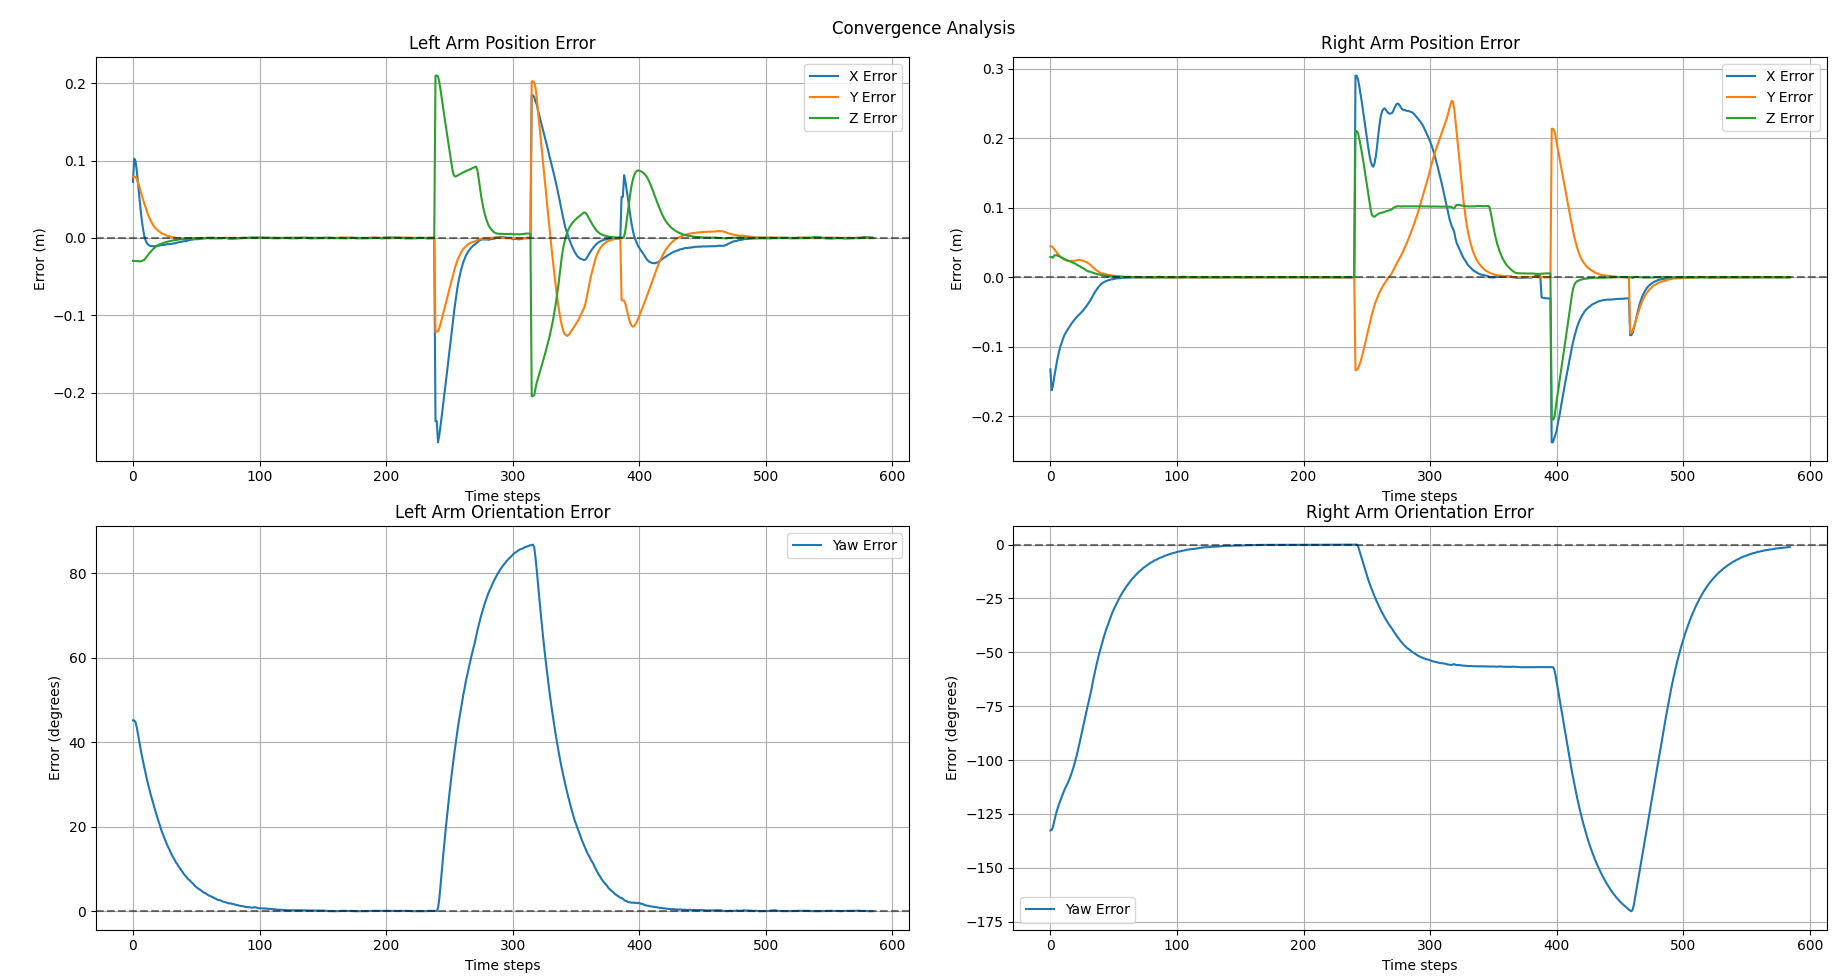
\includegraphics[width=0.9\linewidth]{Images/iapf/convergence_without_home.jpg}
\caption{Position and orientation error convergence without home-seeking active: position
oscillates for a visibly longer interval before settling, while orientation, controlled
independently, still converges comparably to Figure~\ref{fig:iapf_error_with}~\citep{surya2025iapf}.}
\label{fig:iapf_error_without}
\end{figure}

The corresponding error-convergence plots, Figure~\ref{fig:iapf_error_with} against
Figure~\ref{fig:iapf_error_without}, show the same effect in the position and orientation error
signals directly: the three-way equilibrium converges in a single transient per waypoint, while the
two-way formulation's position error oscillates for a visibly longer interval before settling,
despite the orientation loop, controlled independently by
Equation~\eqref{eq:iapf_angular}, converging comparably in both cases, confirming that the
instability is specific to the translational force balance rather than the coupled controller as a
whole.

\begin{figure}[htbp]
\centering
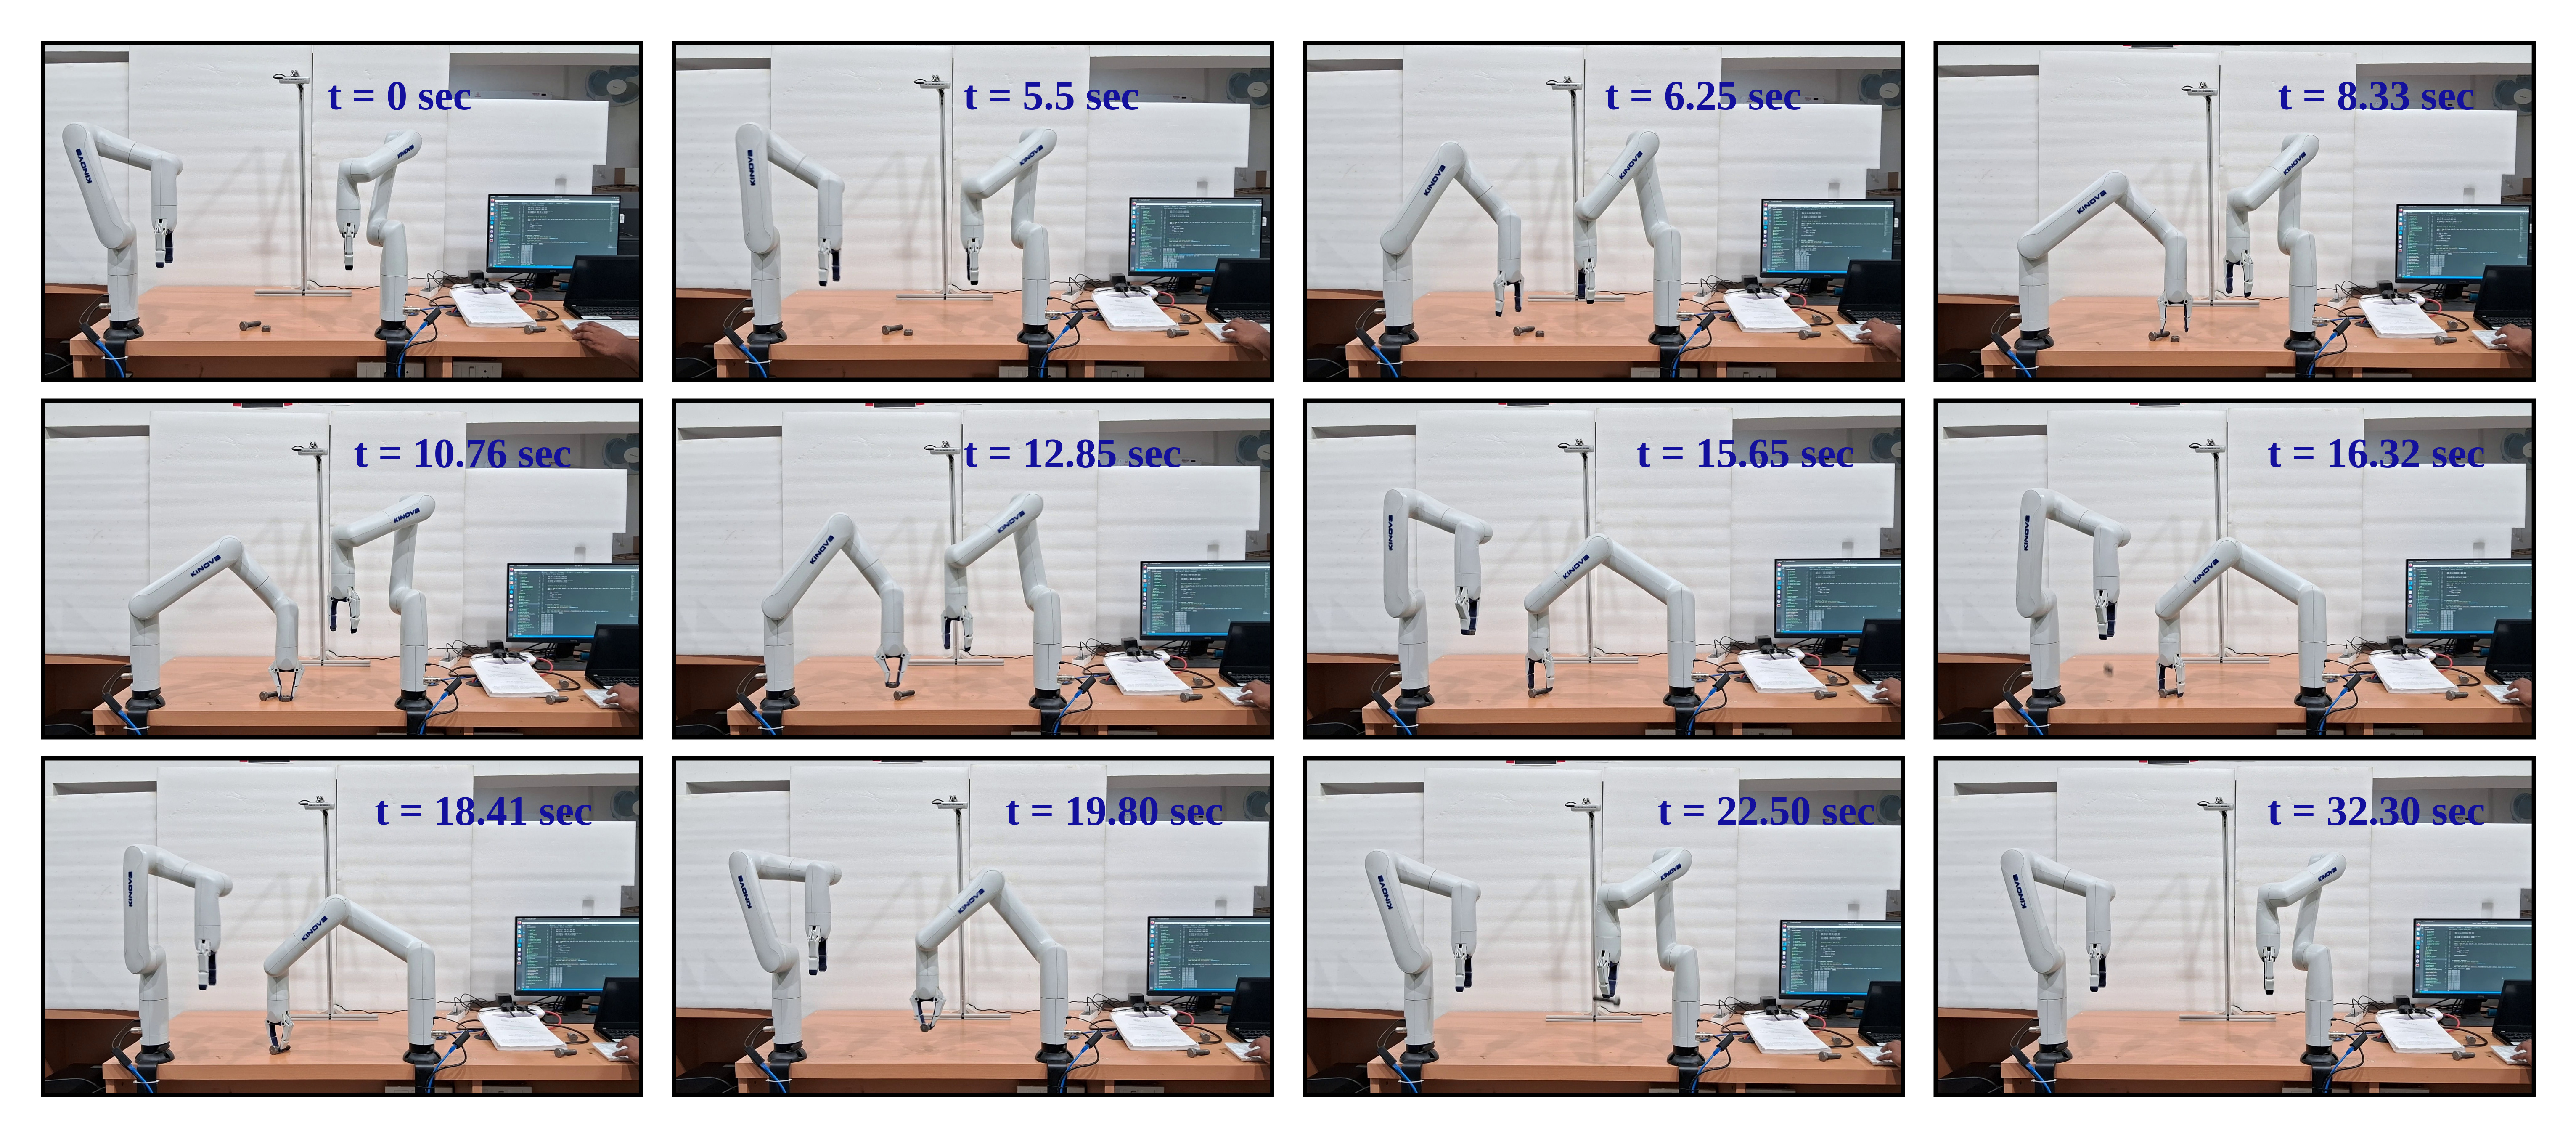
\includegraphics[width=\linewidth]{Images/iapf/sequential_with_home.jpg}
\caption{Sequential demonstration of the priority-lock mechanism with the three-way equilibrium:
the left arm gets priority at close range ($t=6.25$\,s), picks its object while the right arm waits
at a clear transition point ($t=8.33$\,s), the right arm then picks
($t=15.66$\,s), and both arms complete their drops in
turn~\citep{surya2025iapf}.}
\label{fig:iapf_seq_with}
\end{figure}

\begin{figure}[htbp]
\centering
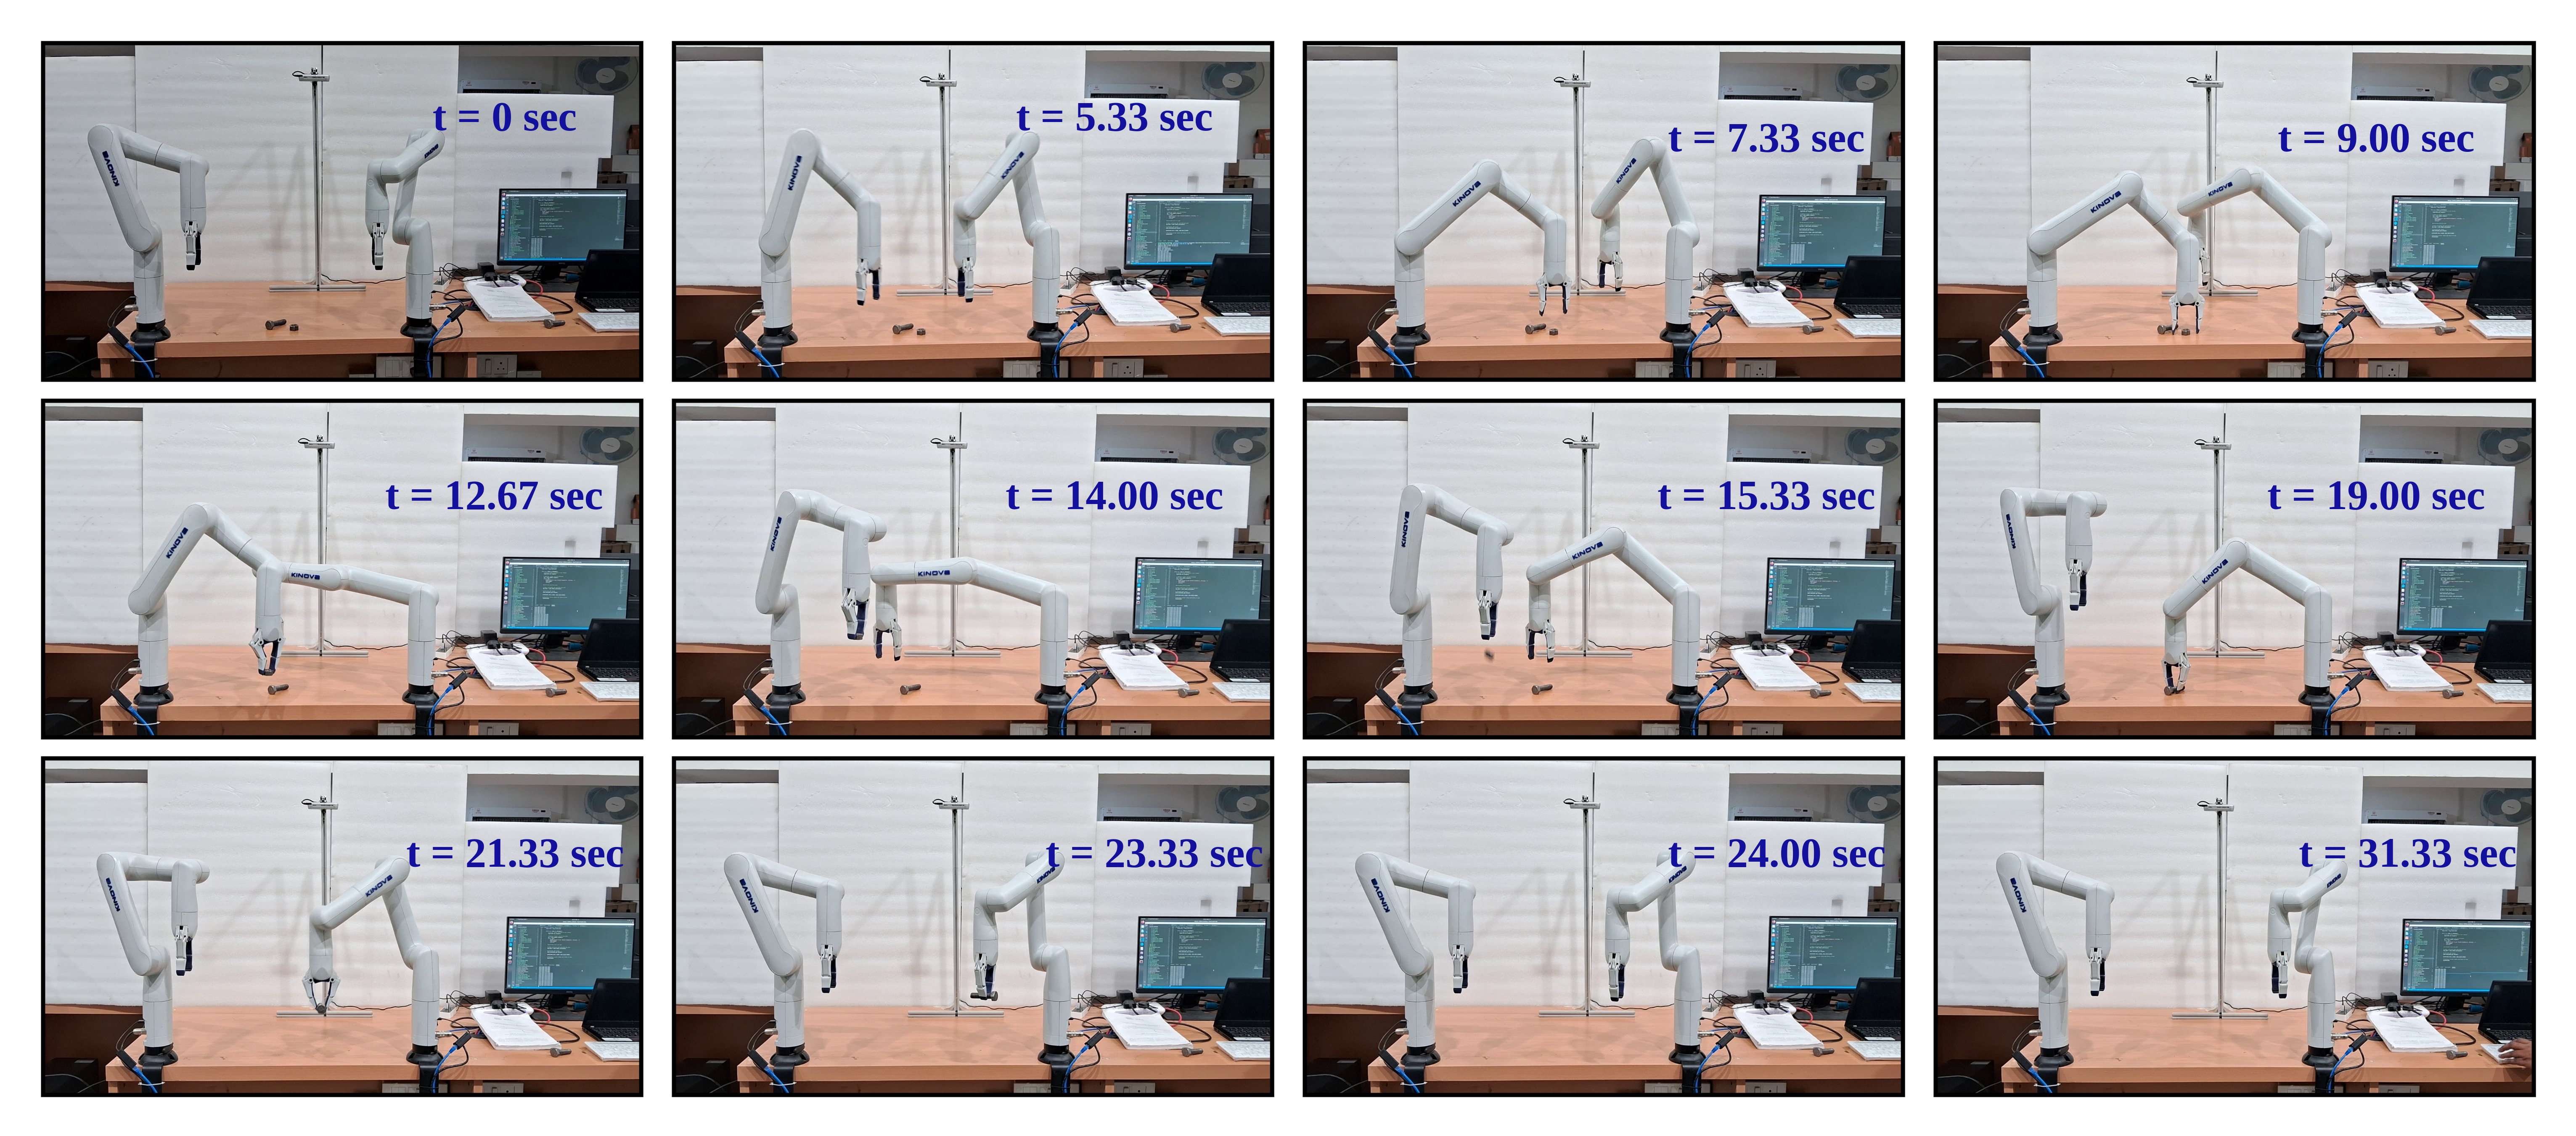
\includegraphics[width=\linewidth]{Images/iapf/sequential_without_home.jpg}
\caption{Sequential demonstration of the same conflict without the three-way equilibrium: the left
arm gets priority at close range ($t=7.33$\,s), but the right arm is pushed far from its target by
the unopposed repulsive spike, bringing the two arms close to collision by
$t=14$\,s~\citep{surya2025iapf}.}
\label{fig:iapf_seq_without}
\end{figure}

Figure~\ref{fig:iapf_seq_with} and Figure~\ref{fig:iapf_seq_without} show this qualitatively as a
sequence of hardware frames: with the three-way equilibrium, the two arms maintain clear spatial
separation throughout the handoff; without it, the repulsion spike pushes the unlocked arm far
enough off its intended path that the two arms come close to colliding, the exact failure mode gap
G4 identifies as endemic to the traditional two-force APF formulation in asymmetric dual-arm
settings.

Across this validation, the fixed nut-left/bolt-right assignment of
Section~\ref{sec:iapf_priority} was sufficient to demonstrate that the three-way equilibrium and its
priority-lock critical-state switching solve the motion-planning half of dual-arm coordination.
What it leaves unaddressed is that the assignment itself is fixed rather than adaptive: precisely
gap G5, which Chapter~\ref{chap:task_allocation} takes up next, reusing the iAPF controller
developed in this chapter entirely unchanged as its execution layer.
